\chapter{Funktionale Analyse der bestehenden Web Content Management Systeme}


\section{Vorbetrachtungen}
Der 2006 eingeleitete Hype um das Ruby on Rails Framework hat dazu geführt, dass viele Entwickler mit der Konzeption und Umsetzung zahlreicher verschiedener Rails-Anwendungen begonnen haben. So entstanden auch im Bereich der Web Content Management Systeme zahlreiche Projekte. Ein Großteil der Vorhaben blieb jedoch in der Konzeptionsphase stecken oder die Entwicklung wurde nach wenigen Jahren eingestellt. Die Ursachen sind dabei vor allem dem Entwicklungsumfeld von Rails und dem Framework selbst geschuldet:


\begin{description}
\item[Schnellebigkeit]\mbox{~}\\*
Die Entwicklung des Ruby on Rails Frameworks unterliegt einem ständigen Wandel und erfordert eine ständige Anpassung des Programmierers an neue Technologien und Konzepte.
\item[Interessenwandlung der Entwickler]\mbox{~}\\*
Die elegante Programmierung mit Ruby und die vielfältigen Möglichkeiten des Ruby on Rails Frameworks erleichtern die Umsetzung verschiedenster Projektideen.
Es ist daher schneller möglich, dass sich Entwickler nach einiger Zeit mit anderen Projekten beschäftigen und bestehende Projekte vernachlässigen\footnote{Im Anhang der Arbeit findet sich eine Übersicht zu ermittelten Rails 2 und 3 Web Content Management Systemen. Diese sind zum Teil seit einigen Jahren nicht mehr weiterentwickelt wurden.}.
\end{description}

Die Realisierung eines stabilen Web Content Management Systems auf Basis von Ruby on Rails wird durch diese Faktoren erschwert und erfordert ein entsprechend tragfähiges Konzept sowie planendes Vorgehen der Projektiniziatoren.

Die hier aufgeführten Projekte Alchemy CMS, Browser CMS, Locomotive CMS und Refinery CMS repräsentieren daher die zum Zeitpunkt der Erstellung dieser Arbeit vielversprechendsten Rails-Implementierungen eines Web Content Management Systems. Trotz alldem ist anzumerken, dass sich diese Systeme, im Gegensatz zu anderen etablierten Web Content Management Systemen wie Typo3 und Drupal, noch am Anfang ihrer Entwicklungsgeschichte befinden.
\newline
\newline
Um die Zahl der zu untersuchenden WCMS einzuschränken, wurden folgende Mindestanforderungen für existierende Rails-Anwendungen festgelegt:
\begin{description}
\item[Open Source Software]\mbox{~}\\*
Die hier ermittelten WCM-Systeme sind vollständige Open Source Lösungen. Ihre Veröffentlichung unterliegt dabei den in der Open Source Bewegung üblichen Lizenzen der Freien Software bzw. der Open Source Initiative (OSI).
\item[Rails 3 Kompatibilität]\mbox{~}\\*
Die Veröffentlichung von Rails 3 brachte vielen Verbesserungen hinsichtlich der Modularität von Rails-Anwendungen. Kern-Komponenten des Frameworks (z.B. die Persistenz-Schicht Active Record) können nun mit geringem Aufwand gegen andere Implementierungen ausgetauscht werden. Die so erreichte Flexibilität soll auch bei der Integration eines Rails WCM-Systems zur Verfügung stehen.	Weiterhin sichert die Verwendung der aktuellsten Framework-Version die 	Unterstützung moderner Technologien und Entwicklungen innerhalb der implementierten WCMS ab.
\item[Aktive Entwicklung]\mbox{~}\\*
Die stetige, aktive Entwicklung an einem Open Source Projekt ist ein Merkmal für die Akzeptanz einer Software. Sie ist zusätzlich ein Beweis für das Engagement der beteiligten Programmierer. Eine in diesem Umfeld entstehende Software bietet daher entsprechend höheres Potenzial. Die  hier ausgewählten Systeme erfüllen diese Forderung.
\newpage
\item[Unterscheidung in Front- und Backend]\mbox{~}\\*
WCM-Systeme unterscheiden zwischen Frontend- und Backend-Funktionalität. Das Frontend wird durch die eigentliche Internetseite repräsentiert, die mit Hilfe des Systems erzeugt wird. Im Backend können Anwender Inhalte zentral einpflegen und verwalten.
Die ausgewählten Implementierungen verfügen über eine solche konzeptionelle Trennung.
\end{description}

\section{Bezugsquellen}

Trotz der steigenden Bekanntheit von Ruby on Rails existiert zum Zeitpunkt der Anfertigung dieser Arbeit keine Fachliteratur, die sich mit den Möglichkeiten des Web Content Managements in Rails auseinandersetzt. Vielmehr sind folgende Schwerpunktsetzungen bei den verschiedenen Autoren festzustellen:
\begin{description}
\item[Grundlagenbücher]\mbox{~}\\*
Sie dienen als Einführung in Rails und verdeutlichen an Hand einfacher Anwendungen die Arbeitsweise mit dem Ruby on Rails Framework.
\item[Fortgeschrittene Techniken mit Ruby on Rails]\mbox{~}\\*
Rails Kern-Entwickler stellen ihre Erfahrungen mit dem Framework dar und geben Lösungsansätze für größere Unternehmensstrukturen und Projekte. Häufig vertiefte Themen sind dabei Skalierung, Performance und Refactoring.
\end{description}
Zur Ermittlung existierender Ruby on Rails Open Source WCMS-Software mussten daher alternative Informationsquellen herangezogen werden, die im folgenden kurz beschrieben werden sollen:
\begin{description}
\item[Anfragen im offiziellen IRC Channel von Ruby on Rails]\mbox{~}\\*
Der Ruby on Rails IRC Channel ermöglicht einen konstruktiven Austausch von Rails-Entwicklern zu verschiedenen Bereichen des Rails-Frameworks. Mit der Hilfe mehrerer hundert Nutzer täglich können so Probleme und Anfragen sehr umfassend beantwortet werden. Der Ruby on Rails Channel ist erreichbar unter \#rubyonrails.
\item[RubyGems.org]\mbox{~}\\*
Bibliotheken können die Funktionalität von Ruby enorm erhöhen. Zur Verbreitung dieser im Internet existiert u.a. der Ruby Online Community Anbieter RubyGems.org, der über 30.000 Erweiterungspakete verschiedenster Entwickler im Internet zum Download anbietet.
Der Dienst verfügt über eine ausführliche Suchfunktion, mit der gezielt nach bestimmten Bibliotheken gesucht werden kann. Neben einer kurzen Projektbeschreibung und Informationen zum Entwickler wird jedem Projekt ein Datum der letzten Aktualisierung zugeordnet. Der Entwicklungsstand eines Pakets kann so besser eingeschätzt werden. RubyGems.org stellt daher einen wichtigen Startpunkt zur Ermittlung existierender Ruby on Rails WCMS dar.
\begin{figure}[!h]
\begin{center}
\label{fig.rubygems}
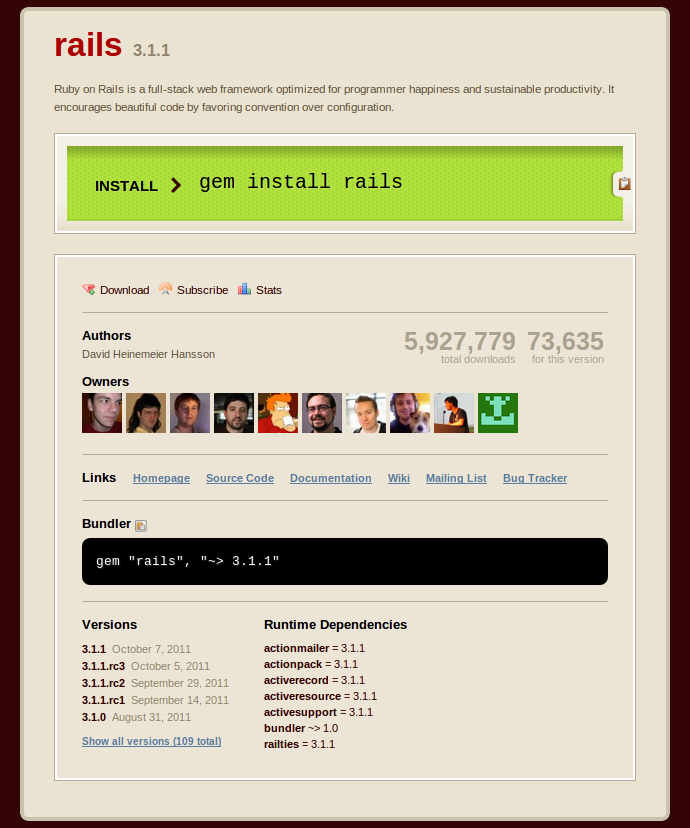
\includegraphics[scale=0.3]{images/analyse/rubygems/railsonrubygems.png}
\caption{Ruby Gems mit aufgelisteten Informationen zum aktuellen Rails 3.1}
\end{center}
\end{figure}
\newpage
\item[Github.com]\mbox{~}\\*
Github.com ist ein Online-Netzwerk und Webhosting-Dienst für Programmierer. Nutzer können dort ihre individuellen Programme, umgesetzt in beliebigen Programmiersprachen, kostenlos\footnote{Die Einrichtung eines kostnpflichtigen, privaten Github-Repositories ist ebenfalls möglich.}  veröffentlichen.
Schlüsseltechnologie des Netzwerkes ist das Versionsverwaltungssystem Git\footnote{PRojektseite: \href{http://git-scm.com/}{http://git-scm.com/}}, welches Änderungen am Quellcode des Projektes festhält. Zusätzlich erlaubt es anderen Programmierern, bestehende Projekte zu kopieren und eigenständig weiterzuentwickeln. Anschließend können diese wieder zu einem Gesamtprojekt verschmolzen werden.
Die Symbiose zwischen den Funktionalitäten von Git und den zahlreichen Interkationsmöglichkeiten der Platform erschaffen eine Entwicklungsumgebung, in der ein schneller und effektiver Austausch zwischen Programmierern und Projekten stattfinden kann.
Innerhalb der Ruby on Rails Community hat sich Github zu einer zentralen Anlaufstelle für Rails-Programmierer entwickelt und besitzt daher zur Ermittlung bestehender Web Content Management Systeme entscheidende Relevanz.
\begin{figure}[!h]
\begin{center}
\label{fig.github}
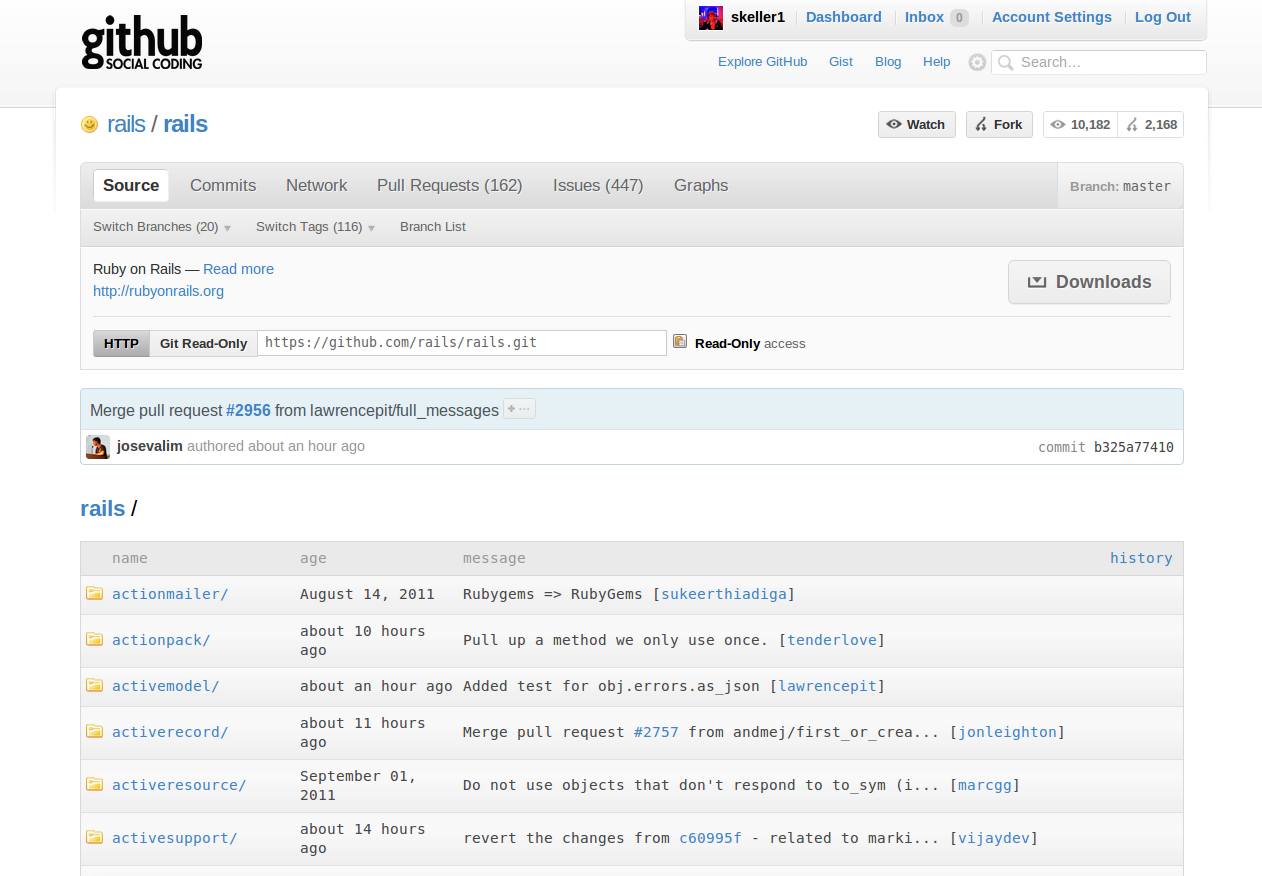
\includegraphics[scale=0.3]{images/analyse/github/github.png}
\caption{Beispiel für ein öffentliches Projekt auf Github.com: Das ausgewählte Projekt ist Rails 3}
\end{center}
\end{figure}
\end{description}

%ALCHEMY BEGIN
\pagebreak
\section{Vorstellung Alchemy CMS}
Unter der Leitung der Hamburger Firma \emph{macabi} wurde 2007 die proprietäre CMS Software \emph{WashAPP} veröffentlicht. Nach der Insolvenz der Entwickler wurde das System zu nächst weiterverkauft (dabei erfolgte die Umbennung in \emph{Webmate}), bevor es 2010 letztendlich als Open Source Software Alchemy CMS an die Öffentlichkeit übergeben wurde. Die Weiterentwicklung übernimmt seitdem die Hamburger Internetagentur \emph{magiclabs*}\footnote{Homepage: \href{http://magiclabs.de/home}{http://magiclabs.de/home}} um die Entwickler Thomas von Deyen, Robin Böning und Carsten Fregin. Die aktuelle Version 1.6.0 steht als Rails 2 und 3 Umsetzung\footnote{Der Rails 3-Entwicklungszweig von Alchemy befindet sich noch im Beta-Stadium.} zur Verfügung.
\begin{table}[!h]
\caption{Steckbrief Alchemy CMS}
\begin{tabular}[!ht]{|l|l|l|}
\hline
\textbf{Aktuelle Version} & \multicolumn{2}{p{10cm}|}{1.6.0} \\
\hline
\textbf{Lizenz} & \multicolumn{2}{p{10cm}|}{GPLv3} \\
\hline
\textbf{Projektseite} & \multicolumn{2}{p{10cm}|}{\href{http://alchemy-cms.com}{http://alchemy-cms.com}} \\
 & \multicolumn{2}{p{10cm}|}{\href{https://github.com/magiclabs/alchemy}{https://github.com/magiclabs/alchemy}} \\
\hline
\textbf{Quellcode} & \multicolumn{2}{p{10cm}|}{\href{https://github.com/magiclabs/alchemy}{https://github.com/magiclabs/alchemy}} \\
\hline
\textbf{IRC-Channel} & \multicolumn{2}{p{10cm}|}{nicht vorhanden} \\
\hline
\textbf{API Dokumentation} & \multicolumn{2}{p{10cm}|}{nicht verfügbar} \\
\hline
\textbf{Forum} & \multicolumn{2}{p{10cm}|}{\href{http://groups.google.com/group/alchemy-cms}{http://groups.google.com/group/alchemy-cms}} \\
\hline
\textbf{Demoversion} & Frontend & \href{http://demo.alchemy-cms.com}{http://demo.alchemy-cms.com} \\
\cline{2-3}
& Backend & \href{http://demo.alchemy-cms.com/admin}{http://demo.alchemy-cms.com/admin} \\
\cline{2-3}
& Login & demo \\
\cline{2-3}
& Passwort & demo \\
\hline
\textbf{Verwendete Technologien} & \multicolumn{2}{p{10cm}|}{Ruby on Rails 3.0.x, HTML, jQuery und jQueryUI, TinyMCE - Javascript WYSIWYG Editor, SWFUpload} \\
\hline
\textbf{Projektbeschreibung} & \multicolumn{2}{p{10cm}|}{Alchemy ist ein unglaubliches Content Managment System, welches sich gut in Rails integrieren lässt. – Absolut flexibel und kraftvoll.} \\
\hline
\textbf{Philosophie} & \multicolumn{2}{p{10cm}|}{Der Benutzer des Systems muss nur Inhalte erstellen und ändern können} \\
& \multicolumn{2}{p{10cm}|}{Formatierung von Überschriften, Bildpositionierung und -berechnung sind Aufgaben des Entwicklers, nicht die des Redakteurs}\\
\hline
\textbf{Zielgruppe} & \multicolumn{2}{p{10cm}|}{Privatnutzer, Kleinstunternehmen} \\
\hline
\end{tabular}
\end{table}

\subsection{Funktionsprinzipien}
Das Backend von Alchemy CMS verfügt u.a. über die Bereiche Seiten, Sprachen, Benutzer und Bibliothek:
\begin{figure}[!h]
\begin{center}
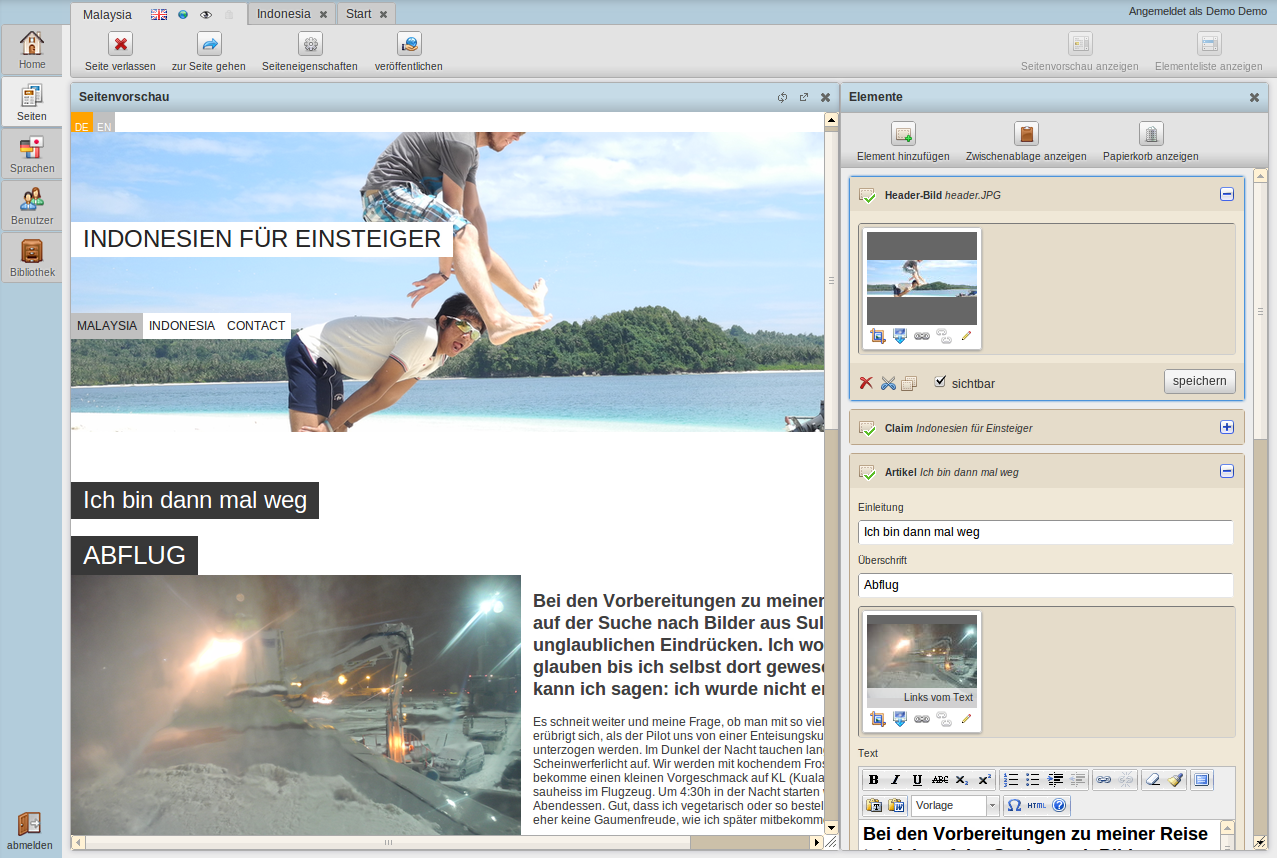
\includegraphics[scale=0.3]{images/analyse/alchemy/inhalte.png}
\caption{Backend-Ansicht von Alchemy CMS mit geöffnerter Seitenvorschau und Elementebearbeitung}
\label{alchemybackend}
\end{center}
\end{figure}

\begin{description}
\item[Home]\mbox{~}\\*
Nach einer erfolgreichen Anmeldung im Backend bildet das Home-Modul eine Art Startseite, in der der Nutzer über die letzten Aktivitäten des Systems informiert wird (z.B. Auflistung der zuletzt editierten Inhalte).
\item[Seiten]\mbox{~}\\*
Im Seiten-Modul des Backends findet die Verwaltung aller im System angelegter Seiten und deren Inhalte statt. Eine abgebildete Baumstruktur ermöglicht dabei einen Überblick über die verwalteten Seiten des Systems. Im Bearbeitungsmodus bietet Alchemy CMS darüber hinaus eine Aufteilung der Ansicht in einen Vorschaubereich, der die aktuell ausgewählte Seite mit ihren tatsächlichen Inhalten anzeigt, und einem Elemente-Bereich, der die auf der Seite verfügbaren Inhalselemente angibt und editierbar macht (Abb. \ref{alchemybackend}).
\item[Sprachen]\mbox{~}\\*
Diese Modul ermöglicht die komfortable Verwaltung der in Alchemy CMS verfügbaren Frontend-Sprachen. Eine Alchemy Standard-Installation enthält bereits die Sprachen Deutsch und Englisch.
\item[Benutzer]\mbox{~}\\*
Das Benutzer-Modul ist die zentrale Anlaufstelle zur Verwaltung der am System registrierten Administratoren, Autoren und Redakteure sowie ihrer jeweiligen Befugnisse innerhalb des CMS.
\item[Bibliothek]\mbox{~}\\*
Bilder und andere Dateien werden in Alchemy CMS über das Bibliotheken-Modul verwaltet. Es ermöglicht die Auflistung aller im System zur Verfügung stehenden Ressourcen. Zusätzlich stehen Funktionen zum Hochladen, Editieren und Löschen von Ressourcen zur Verfügung.
\end{description}
\subsection{Erweiterungen}
Alchemy kann durch die Erstellung von Plugins in seiner Funktionalität erweitert werden. An Hand einer definierten API wird ein Grundgerüst angeboten, mit deren Hilfe Erweiterungen bequem in alle Teile des Systems integriert werden können. Ein Plugin kann so entweder als neues Backend-Modul umgesetzt werden (es erscheint in Form eines neuen Menüeintrages im linken Bereich des Backends) oder neue Inhaltselemente zur Verfügung stellen, die dann innerhalb der Seitenbearbeitung als auswählbarer Inhaltstyp zur Verfügung stehen (Abb. \ref{img.alchemycontenttypes}).
\newline
\newline
Folgende offiziellen Erweiterungen sind ebenfalls verfügbar:
\begin{itemize}
\item
alchemy-mailings\footnote{Komponenten-Download: \href{https://github.com/magiclabs/alchemy-mailings}{https://github.com/magiclabs/alchemy-mailings}}: Ermöglicht die Erstellung und Verwaltung von Newsletters im Backend des Systems.
\item
alchemy-standard-set\footnote{Komponenten-Download: \href{ https://github.com/magiclabs/alchemy-standard-set}{ https://github.com/magiclabs/alchemy-standard-set}}: Enthält CSS-Formatierungen für die in Alchemy verfügbaren Standard-Inhaltselemente.
\end{itemize}

\begin{figure}[!h]
\begin{center}
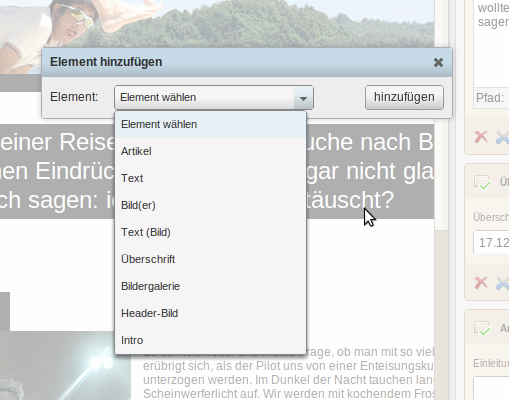
\includegraphics[scale=0.6]{images/analyse/alchemy/dialoginhaltselement.png}
\caption{Standardset von Inhaltselementen in Alchemy CMS}
\label{img.alchemycontenttypes}
\end{center}
\end{figure}



\subsection{Verwendete Technologien}
Schwerpunkttechnologien der Nutzeroberfläche von Alchemy CMS sind die an Hand von Rails erzeugten HTML-Views und darin eingebundene JavaScript-Dateien, die mit Hilfe des JavaScript Frameworks jQuery erstellt wurden.
Das Seiten-Modul greift zusätzlich auf die jQuery UI Bibliothek zurück, die vorgefertigte Elemente zur Erstellung von Dialogboxen und dem Tabulator-Menü liefert.
Der bei einigen Inhaltselementen verfügbare WYSIWJG-Javascript Editor TinyMCE ermöglicht die Formatierung einzelner Inhalte und das Einfügen von vorgefertigtem HTML.
Ein Hochladen von Ressourcen erfolgt in Alchemy über ein herkömmliches HTML Upload-Feld oder den integrierten Adobe Flash Uploader, der somit auch das Einstellen mehrerer Medien in einem Schritt ermöglicht.
%ALCHEMY END


%Browser BEGIN


\newpage
\section{Vorstellung Browser CMS}
Browser CMS ist ein Open Source Web Content Management System der US-amerikanischen Agentur BrowserMedia mit Sitz in Bethesda, Maryland. Im Gegensatz zum aktuellen Versionszweig 3.x des Systems wurden die Vorgängerversionen (Versionen 1.x und 2.x) mit Hilfe der Java Programmiersprache umgesetzt.
Auf Grund geänderter Marktsituation entschied sich BrowserMedia jedoch 2009 dazu, alle weiteren Versionen des CMS auf Grundlage des Rails Frameworks\footnote{Ausführliche Informationen zum Übergang von Java auf Rails können unter folgender Quelle nachvollzogen werden: href{http://tinyurl.com/6eayba7
}{http://tinyurl.com/6eayba7}} zu entwickeln. Zusätzlich erfolgte der Umstieg auf die GPLv3-Lizenz, die eine freie Verwendung der Software ermöglicht.
Eine online verfügbare Testversion des Systems wird von BrowserMedia nicht angeboten. Um dennoch die Funktionalität des Systems zu demonstrieren, wurde eine Installation  von Browser CMS 3.3.1 eingerichtet\footnote{Die Upload-Funktion des CMS wurde auf Grund zu geringer Server-Ressourcen deaktiviert.}.
\begin{table}[!h]
\caption{Steckbrief Browser CMS}
\begin{tabular}[!ht]{|l|l|l|}
\hline
\textbf{Aktuelle Version} & \multicolumn{2}{p{10cm}|}{3.3.1} \\
\hline
\textbf{Lizenz} & \multicolumn{2}{p{10cm}|}{GPLv3} \\
\hline
\textbf{Projektseite} & \multicolumn{2}{p{10cm}|}{\href{http://browsercms.org}{http://browsercms.org}} \\
\hline
\textbf{Quellcode} & \multicolumn{2}{p{10cm}|}{\href{https://github.com/browsermedia/browsercms
}{https://github.com/browsermedia/browsercms}} \\
\hline
\textbf{IRC-Channel} & \multicolumn{2}{p{10cm}|}{nicht vorhanden} \\
\hline
\textbf{API Dokumentation} & \multicolumn{2}{p{10cm}|}{\href{http://rubydoc.info/gems/browsercms/
}{http://rubydoc.info/gems/browsercms/}} \\
\hline
\textbf{Forum} & \multicolumn{2}{p{10cm}|}{\href{http://groups.google.com/group/browsercms}{http://groups.google.com/group/browsercms}} \\
\hline
\textbf{Demoversion} & Frontend & \href{http://diplomabcms.heroku.com/}{http://diplomabcms.heroku.com/} \\
\cline{2-3}
& Backend & \href{http://diplomabcms.heroku.com/cms}{http://diplomabcms.heroku.com/admin} \\
\cline{2-3}
& Login & demo \\
\cline{2-3}
& Passwort & demo \\
\hline
\textbf{Verwendete Technologien} & \multicolumn{2}{p{10cm}|}{Ruby on Rails 3.0.x, HTML, jQuery und jQueryUI, diverse jQuery Plugins ,WYSIWYG-HTML-Editor CKEditor} \\
\hline
\textbf{Projektbeschreibung} & \multicolumn{2}{p{10cm}|}{Menschliches Content Management mit Ruby on Rails 3 Unterstützung} \\
%\hline
%\textbf{Philosophie} & \multicolumn{2}{p{10cm}|}{Redakteuren soll es ermöglicht werden, ohne HTML- und Rails-Kenntnisse eine Internetseite zu verwalten} \\
\hline
\textbf{Zielgruppe} & \multicolumn{2}{p{10cm}|}{Privatnutzer, Kleine und mittelständige Unternehmen mit einer hohen Anzahl von Redakteuren} \\
\hline
\end{tabular}
\end{table}
\subsection{Funktionsprinzipien}

Innerhalb des Backend (Abb. \ref{browserbackend}) von Browser CMS kann der angemeldete Nutzer auf alle wichtigen Funktionsbereiche des Systems zugreifen:


\begin{figure}[!h]
\begin{center}
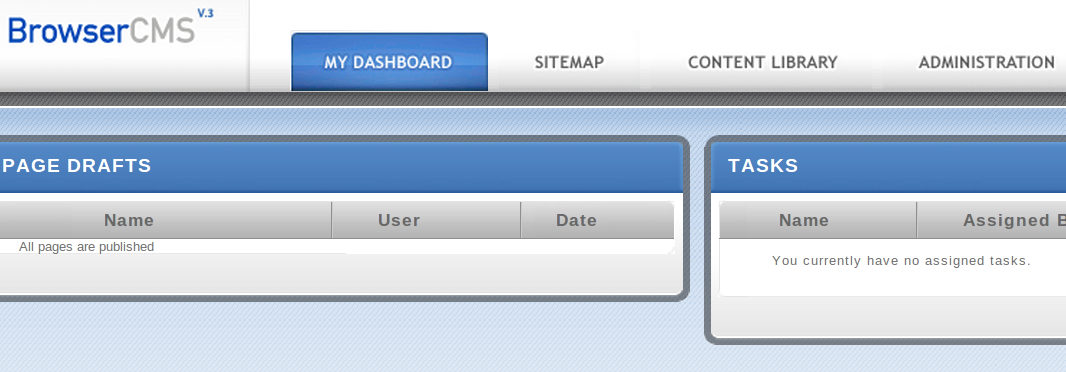
\includegraphics[scale=0.3]{images/analyse/browser/backend.png}
\caption{Backend-Ansicht von Browser CMS}
\label{browserbackend}
\end{center}
\end{figure}


\begin{description}
\item[Dashboard]\mbox{~}\\*
Das Dashboard gibt eine Übersicht über die zuletzt vom Nutzer bearbeiteten Seiten sowie eine Auflistung der vom Anwender noch zu erledigenden Aufgaben.
\item[Sitemap]\mbox{~}\\*
Das Sitemap-Menü ermöglicht die Darstellung aller im System existierenden Seiten in einer Baumstruktur sowie die Bearbeitung aller Informationen zu einer einzelnen Seite. U.a. kann der Titel, das verwendete Template und verschiedene Meta-Informationen verändert werden.
\item[Content Library]\mbox{~}\\*
In der Content Library von Browser CMS können alle existierenden Inhaltselemente sortiert nach Inhaltstyp (z.B. Text, File, Image) aufgelistet und bearbeitet werden.
\item[Administration]\mbox{~}\\*
Im Administrator-Bereich des Systems werden alle Gruppen und Nutzer des Backend und der Internetseite verwaltet. Zusätzlich können die für die einzelnen Seiten und Inhaltselemente definierten Templates aufgelistet und bearbeitet werden.
\end{description}

\begin{figure}[!h]
\begin{center}
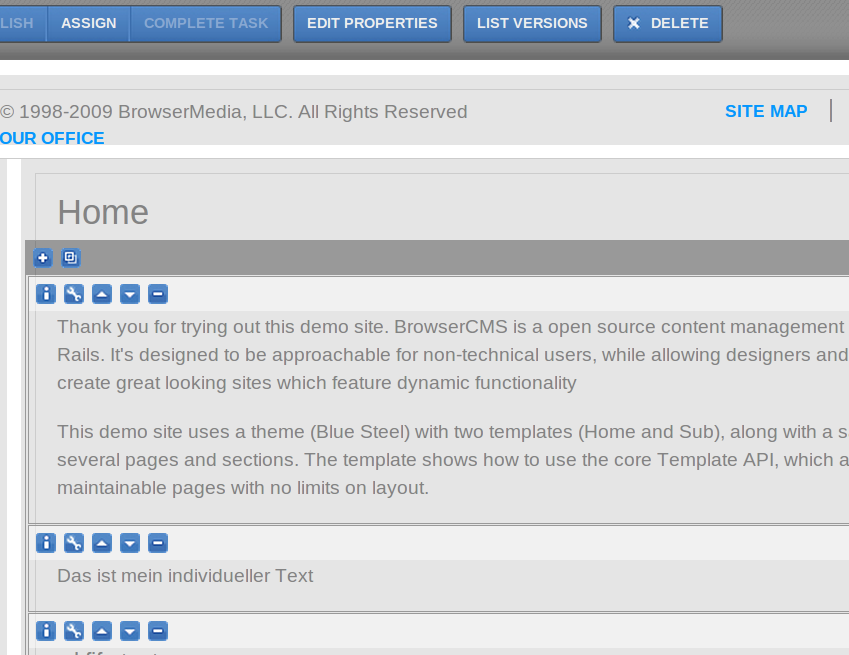
\includegraphics[scale=0.3]{images/analyse/browser/frontendangemeldet.png}
\caption{Ausgewählte Seite im Bearbeitungsmodus und aktiviertem Visual Editor}
\label{browserpageedit}
\end{center}
\end{figure}
Die Erstellung und Darstellung von Inhalten in Browser CMS wird durch folgende 2 Prinzipien realisiert:
\begin{description}
\item[Content Blocks]\mbox{~}\\*
Content Blocks sind Sammlungen von Daten mit einer definierten Anzahl an Feldern eines bestimmten Typs (z.B. Textfeld, Datumsfeld). Innerhalb der Content Library können diese verwaltet und angelegt werden.
\item[Portlet\footnote{Der Begriff des Portlets stammt aus der Java-Welt und bezeichnet ursprünglich beliebig kombinierbare Komponenten, die an verschiedenen Positionen auf einer Internetseite bzw. einer Portal-Seite dargestellt werden können.}]\mbox{~}\\*
Portlets sind spezielle Content Blocks, die festlegen, wie bereits existierende Content Blocks (z.B. Text, News) dargestellt werden sollen. Dazu verfügt jedes Portlet über ein im Backend editierbares Template, dass die zuvor ausgewählten Datensätze in dem gewünschten Layout präsentiert (Abb. \ref{browsertagportlet}).

\begin{figure}[!h]
\begin{center}
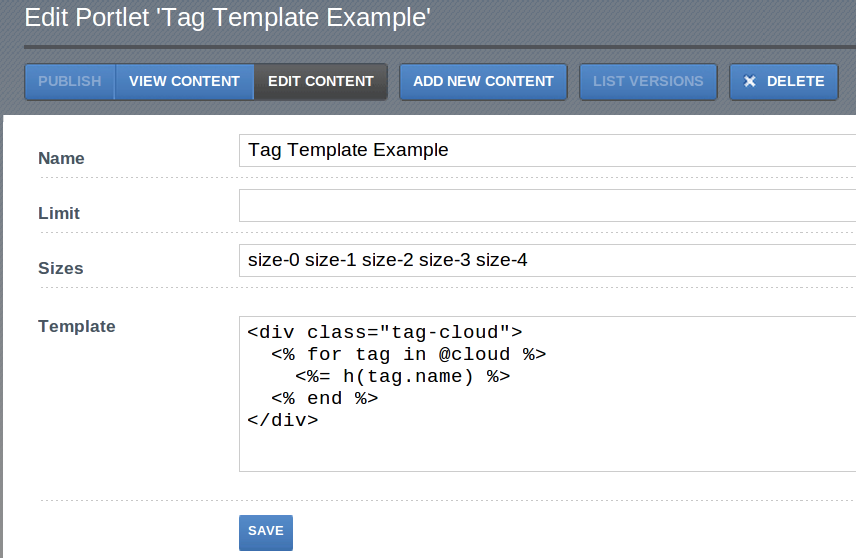
\includegraphics[scale=0.3]{images/analyse/browser/tagportlet.png}
\caption{Tag-Portlet mit Template im Backend von Browser CMS}
\label{browsertagportlet}
\end{center}
\end{figure}


\end{description}

\subsection{Erweiterungen}
Die Funktionalität von Browser CMS kann durch das Hinzufügen von sogenannten Modulen erweitert werden. Diese beinhalten dabei neue Content-Blocks oder vordefinierte Portlets, die in der Content Library des Backends verwaltet werden können. Im Internet stehen zusätzlich folgende vorgefertigten Erweiterungen bzw. Module zur Verfügung\footnote{Eine ausführliche Liste mit allen Erweiterungen findet sich unter folgender Adresse: \href{http://modules.browsercms.org/modules}{http://modules.browsercms.org/modules}}:


\begin{itemize}
\item browsercms-news\footnote{Komponenten-Download: \href{https://github.com/browsermedia/bcms\_news}{https://github.com/browsermedia/bcms\_news}}: Darstellung von kurzen Nachrichten im Frontend der Seite.
\item browsercms-blog\footnote{Komponenten-Download: \href{https://github.com/browsermedia/bcms\_blog}{https://github.com/browsermedia/bcms\_blog}}: Erstellung und Verwaltung von Blog-Einträgen inklusive Kommentar- und Tagging-Funktionalität.
\item browsercms-events\footnote{Komponenten-Download: \href{https://github.com/browsermedia/bcms\_event}{https://github.com/browsermedia/bcms\_event}}: Erstellung und Verwaltung von Event-Einträgen. Diese können wahlweise alle zusammen in einer Listenansicht oder in Einzeldarstellung individuell präsentiert werden.
\item browsercms-rankings\footnote{Komponenten-Download: \href{https://github.com/browsermedia/bcms\_rankings}{https://github.com/browsermedia/bcms\_rankings}}: Erlaubt dem Internetseitenbenutzer eine Bewertung der besuchten Seite abzugeben.
\end{itemize}

\subsection{Verwendete Technologien}

Das komplette Backend von Browsercms wird mit Hilfe von in Rails gerenderten HTML-Views erzeugt. JavaScript kommt lediglich bei der Darstellung verschiedener Feldtypen (z.B. Datumsdialog und Auswahlbox) innerhalb der Contentblöcke und beim Anlegen von Textinhalt durch die Verwendung des JavaScript-WYSIWYG-Editors FCKEditor (Abb. \ref{browsereditor}) zur Anwendung. Dieser ermöglicht die komfortable Formatierung eingestellter Texte sowie die Einbindung von vorformatierten HTML-Inhalten.

\begin{figure}[!h]
\begin{center}
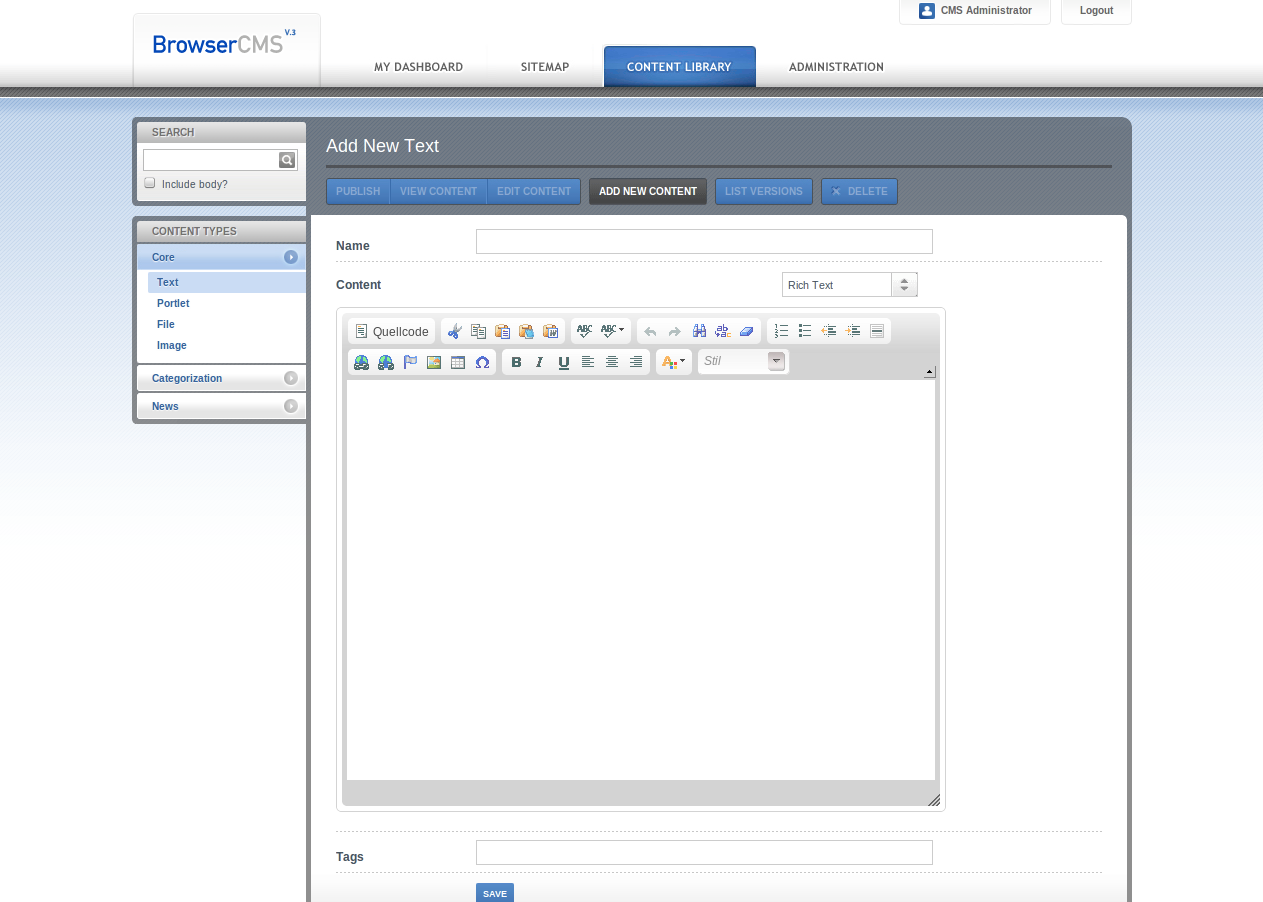
\includegraphics[scale=0.3]{images/analyse/browser/editor.png}
\caption{Erstellung eines neuen Content Blocks Text mit Hilfe des FCKEditor}
\label{browsereditor}
\end{center}
\end{figure}

Die Erstellung der Contentblöcke (Content Blocks) und Portlets wird durch einen in Rails umgesetzten Generatorskript ermöglicht und vereinfacht somit die Erstellung für den Entwickler. Er erzeugt ein komplettes


\lstinputlisting[caption=Aufruf des Generator-Skripts zur Erstellung eines neuen Inhaltselements Produkt]{code/content_block.rb}
%Browser END
\newpage
%Locomotive BEGIN
\section{Vorstellung Locomotive CMS}
Lokomotive CMS ist ein Open Source Content Management System der Ruby on Rails Entwickler Didier Lafforgue und Jacques Crocker sowie dem Designer Sacha Greif. Es wird unter der MIT Lizenz der Open Source Initiative vertrieben und steht in den Rails-Versionen 2 und 3 als Downloadpaket zur Verfügung. Neben den Möglichkeiten der eigenständigen Installation bieten die Initiatoren des Systems auch den kostenpflichtigen Dienst Bushi.do an, der eine automatische Installation von Lokomotive CMS vornimmt und es ermöglicht, nach wenigen Minuten sofort mit der Erstellung der Seite im Browser zu beginnen\footnote{Auf der Projektseite von Lokomotive CMS wird die automatische Installation mit Hilfe von Bushi.do beschrieben: \href{http://www.locomotivecms.com/}{http://www.locomotivecms.com/}}.
\begin{table}[!h]
\caption{Steckbrief Locomotive CMS}
\begin{tabular}[!ht]{|l|l|l|}
\hline
\textbf{Aktuelle Version} & \multicolumn{2}{p{10cm}|}{keine Angabe von Entwicklungsversionen} \\
\hline
\textbf{Lizenz} & \multicolumn{2}{p{10cm}|}{MIT License} \\
\hline
\textbf{Projektseite} & \multicolumn{2}{p{10cm}|}{\href{http://www.locomotivecms.com/}{http://www.locomotivecms.com/}} \\
\hline
\textbf{Quellcode} & \multicolumn{2}{p{10cm}|}{\href{https://github.com/locomotivecms/engine}{https://github.com/locomotivecms/engine}} \\
\hline
\textbf{IRC-Channel} & \multicolumn{2}{p{10cm}|}{\#locomotivecms} \\
\hline
\textbf{API Dokumentation} & \multicolumn{2}{p{10cm}|}{\href{http://rubydoc.info/github/resolve/refinerycms}{http://rubydoc.info/github/resolve/refinerycms}} \\
\hline
\textbf{Forum} & \multicolumn{2}{p{10cm}|}{\href{http://groups.google.com/group/refinery-cms/}{http://groups.google.com/group/refinery-cms/}} \\
\hline
\textbf{Demoversion} & Frontend & \href{http://diplomalocomotive.heroku.com/}{http://diplomalocomotive.heroku.com/} \\
\cline{2-3}
& Backend & \href{http://diplomalocomotive.heroku.com/admin}{http://diplomalocomotive.heroku.com/admin} \\
\cline{2-3}
& Login & demo@demo.de \\
\cline{2-3}
& Passwort & demo123 \\
\hline
\textbf{Verwendete Technologien} & \multicolumn{2}{p{10cm}|}{Ruby on Rails 3.0.x, HTML, jQuery und jQueryUI, diverse jQuery Plugins ,WYSIWYG-HTML-Editor Aloha und TinyMCE, MongoDB, Template Sprache Liquid} \\
\hline
\textbf{Projektbeschreibung} & \multicolumn{2}{p{10cm}|}{Locomotive ist ein Open Source CMS für Rails. Es ist sehr flexibel und unterstützt Heroku und Amazon S3.} \\
\hline
\textbf{Philosophie} & \multicolumn{2}{p{10cm}|}{Verwaltung kleiner Internetseiten} \\
& \multicolumn{2}{p{10cm}|}{Komplexe Inhaltselemente dank MongoDB selbst erstellen}\\
\hline
\textbf{Zielgruppe} & \multicolumn{2}{p{10cm}|}{Privatnutzer, Kleinstunternehmen} \\
\hline
\end{tabular}
\end{table}
\subsection{Funktionsprinzipien}
Locomotive CMS unterscheidet im Backend der Anwendung in folgende 2 Funktionsbereiche:
\begin{description}
\item[Inhalte]\mbox{~}\\*
Im Inhalte-Bereich des Backends werden alle im System angelegten Seiten und Inhaltselemente verwaltet und bearbeitet (Abb. \ref{locomotivebackend}). Die Darstellung jeder einzelnen Seite und der Inhaltselemente kann darüber hinaus durch Angabe eines Templates online verändert werden (mehr dazu in Abschnitt \ref{sec:TechnologienLocomotive}), was eine Umsetzung komplexer Seitenlayouts sicherstellt.
\begin{figure}[!h]
\begin{center}
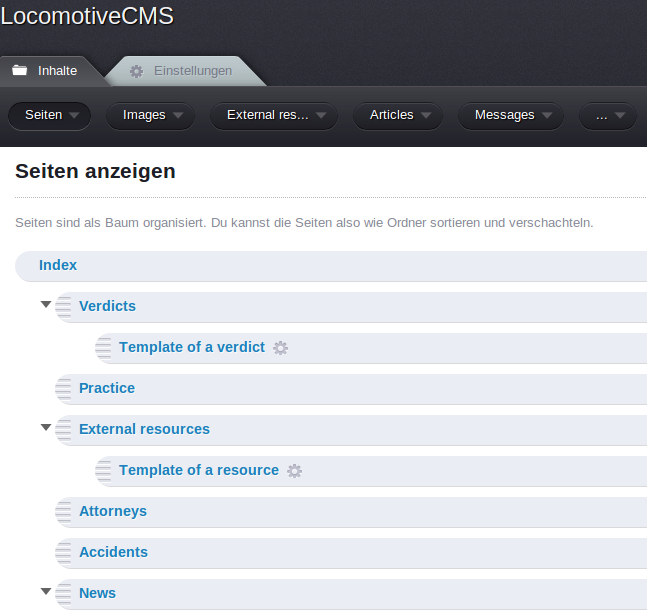
\includegraphics[scale=0.3]{images/analyse/locomotive/backendlocomotive.png}
\caption{Backend von Locomotive CMS mit geöffnetem Seitenbaum.}
\label{locomotivebackend}
\end{center}
\end{figure}
\item[Einstellungen]\mbox{~}\\*
Im Einstellungs-Modul befinden sich die zentralen Funktionen zur Bearbeitung der vorhandenen Backend-Nutzer sowie globaler Locomotive CMS-Einstellungen (registrierte Domains, Import-/Export von Seiten, Bearbeitung von allgemeinen Metainformationen des Systems). Zusätzlich können in einem Template-Bereich einzelne, zentrale Dateien verwaltet werden, die innerhalb des Seitenlayouts der Seite als Gestaltungselemente dienen sollen\footnote{Die für layoutspezifische Verwendung hochgeladenen Dateien werden in Locomotive CMS als Snippets bezeichnet}.
\end{description}
\subsection{Erweiterungen}
\label{sec:ErweiterungenLocomotive}
Erweiterungen werden in Locomotive CMS als Bausteine bezeichnet und repräsentieren individuell zusammengestellte Inhaltselemente. Sie können im Backend von Locomotive CMS über einen komfortablen Bearbeitungsdialog erstellt werden (Abb. \ref{locomotivecontent}). Im Gegensatz zu den hier bereits vorgestellten Systemen werden so keine Programmierkenntnisse der Anwender benötigt. Ebenfalls entfällt der Aufwand zur Installation einer Erweiterung.
\begin{figure}[!h]
\begin{center}
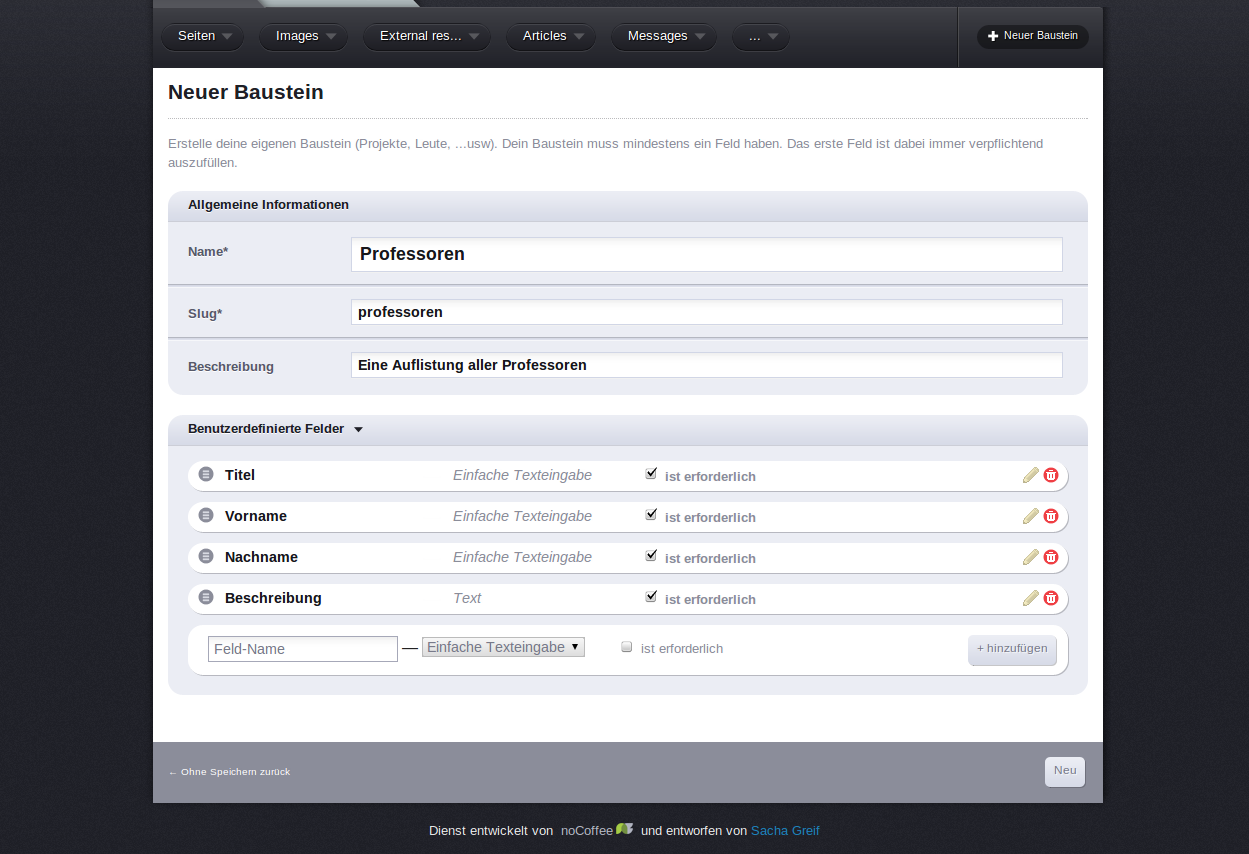
\includegraphics[scale=0.3]{images/analyse/locomotive/customcontent.png}
\caption{Ein im Backend von Locomotive CMS zusammengestelltes Inhaltselement}
\label{locomotivecontent}
\end{center}
\end{figure}
\newpage
Die Inhaltselemente können aus folgenden grundlegenden Feldtypen zusammengebaut werden:
\begin{itemize}
\item
Einfaches Textfeld
\item
Text
\item
Auswahlbox
\item
Checkbox
\item
Datum
\item
Datei
\item
has one (ermöglicht die Zuordnung genau eines anderen Inhaltselements des angegebenen Bausteintyps)
\item
has many (ermöglicht die Auswahl mehrerer anderer Inhaltselemente des angegebenen Bausteintyps)
\end{itemize}

\subsection{Verwendete Technologien}
\label{sec:TechnologienLocomotive}
%Locomotive END
Das Backend von Locomotive CMS besteht aus in Rails gerenderten HTML-Views mit eingebundenen JavaScript-Dateien, die einzelne Funktionalitäten bereitstellen. Das HTML wird dabei zusätzlich durch die Verwendung der JavaScript-Bibliothek Sizzle\footnote{Komponenten-Download: \href{http://sizzlejs.com/}{http://sizzlejs.com/}} manipuliert, die es erlaubt durch Angabe eines CSS-Selektors bestimmte Elemente des HTML zu erfassen.
Zur Erstellung von Templates wird die Ruby Template-Sprache Liquid eingesetzt. Sie hat ihren Ursprung in der kommerziellen Online E-Commerce-Plattform \emph{shopify}\footnote{Liquid ist das Ergebnis einer Extrahierung dieser Funktionalität aus Shopify} und beitet Möglichkeiten der Vererbung und Überschreibung vorheriger definierter Templates.
Der im Backend eingesetzte WYSIWYG-Editor TinyMCE ermöglicht die komfortable Eingabe von Text und HTML-Elementen\footnote{Um den Editor innerhalb der einzelnen Seiten zu aktivieren, müssen im Liqiud-Template der Seite entsprechende Befehle aufgerufen werden. Nach einem erneuten speichern der Seite steht der Editor im Backend zur Verfügung und kann mit Inhalten gefüllt werden.}.


Im Frontend der Seite findet zusätzlich der WYSIWYG-JavaScript-HTML5-Editor Aloha\footnote{Projektseite: \href{http://aloha-editor.org/}{http://aloha-editor.org/}} Verwendung. Er ermöglicht so eine Bearbeitung spezieller Inhaltselemente direkt im Frontend der Seite (Inline-Editing\footnote{Die Entwicklung dieses Features befindet sich noch im Betastatdium und kann noch nicht zuverlässig verwendet werden.}).

\newpage
%Refinery BEGIN
\section{Vorstellung Refinery CMS}
Refinery CMS - in der Kurzform oft als Refinery bezeichnet - ist ein freies Open Source Web Content Management System des neuseeländischen Entwicklerteams Resolve Digital, dessen Entwicklung 2004 durch David Jones eingeleitet wurde. Nach einer fünfjährigen, eingeschränkten Entwicklungsphase, in der nur wenige Bereiche des Systems verbessert wurden, erfolgte am 28. Mai 2009 die Veröffentlichung der ersten Open Source Software Version. In der Folgezeit wurde das CMS durch die Kernentwickler David Jones, Philip Arndt, Steven Heidel und U\'{g}is Ozols auf das aktuelle Rails 3 umgestellt und eine erste stabile Version 1.0.0 veröffentlicht (28. Mai 2011).
\begin{table}[!h]
\caption{Steckbrief Refinery CMS}
\begin{tabular}[!ht]{|l|l|l|}
\hline
\textbf{Aktuelle Version} & \multicolumn{2}{p{10cm}|}{1.0.8} \\
\hline
\textbf{Lizenz} & \multicolumn{2}{p{10cm}|}{MIT License} \\
\hline
\textbf{Projektseite} & \multicolumn{2}{p{10cm}|}{\href{http://refinerycms.com}{http://refinerycms.com}} \\
\hline
\textbf{Quellcode} & \multicolumn{2}{p{10cm}|}{\href{https://github.com/resolve/refinerycms}{https://github.com/resolve/refinerycms}} \\
\hline
\textbf{IRC-Channel} & \multicolumn{2}{p{10cm}|}{\#refinerycms} \\
\hline
\textbf{API Dokumentation} & \multicolumn{2}{p{10cm}|}{\href{http://rubydoc.info/github/resolve/refinerycms}{http://rubydoc.info/github/resolve/refinerycms}} \\
\hline
\textbf{Forum} & \multicolumn{2}{p{10cm}|}{\href{http://groups.google.com/group/refinery-cms/}{http://groups.google.com/group/refinery-cms/}} \\
\hline
\textbf{Demoversion} & Frontend & \href{http://demo.refinerycms.com}{http://demo.refinerycms.com} \\
\cline{2-3}
& Backend & \href{http://demo.refinerycms.com/refinery}{http://demo.refinerycms.com/refinery} \\
\cline{2-3}
& Login & demo \\
\cline{2-3}
& Passwort & demo \\
\hline
\textbf{Verwendete Technologien} & \multicolumn{2}{p{10cm}|}{Ruby on Rails 3.0.x, HTML, jQuery und jQueryUI, WYSIWYG-HTML-Editor Wymeditor, HTML 5 Multi-Upload} \\
\hline
\textbf{Projektbeschreibung} & \multicolumn{2}{p{10cm}|}{Erweiterbares Ruby on Rails „CMS Framework“ mit  Ruby on Rails 3 Unterstützung} \\
\hline
\textbf{Philosophie} & \multicolumn{2}{p{10cm}|}{Realisierung einer benutzerfreundlichen, einfachen Oberfläche} \\
& \multicolumn{2}{p{10cm}|}{Einfaches Hinzufügen von Funktionalität an Hand der in Rails bekannten Entwicklungsabläufe}\\
& \multicolumn{2}{p{10cm}|}{Aktive Community durch Google Group und IRC, die eine schnelle Hilfe ermöglichen}\\
\hline
\textbf{Zielgruppe} & \multicolumn{2}{p{10cm}|}{Privatnutzer, Kleinstunternehmen} \\
\hline
\end{tabular}
\end{table}
\subsection{Funktionsprinzipien}
Das Backend bildet in Refinery CMS die zentrale Anlaufstelle zur Erstellung und Verwaltung aller Inhalte, Einstellungen und Nutzer. Über ein zentrales Menü kann auf die Funktionsmodule des Systems zugegriffen werden, welche im folgenden vorgestellt werden:
\begin{figure}[!h]
\begin{center}
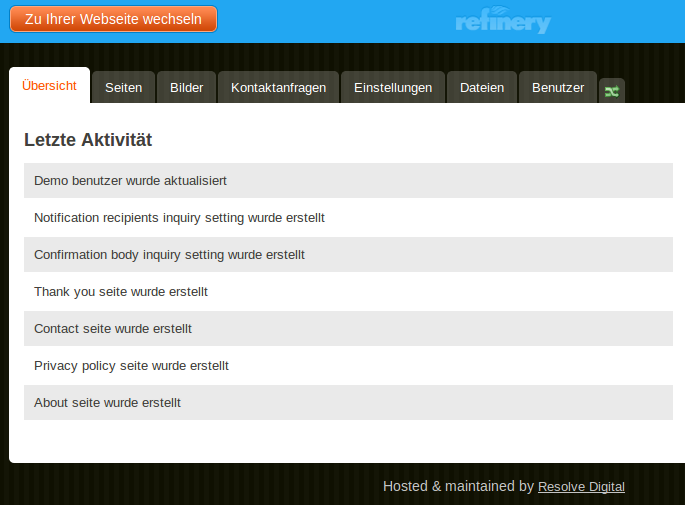
\includegraphics[scale=0.3]{images/analyse/refinery/backendrefinery.png}
\caption{Backend-Ansicht von Refinery CMS}
\label{refinerybackend}
\end{center}
\end{figure}

\begin{description}
\item[Übersichts-Modul]\mbox{~}\\*
Nach der Anmeldung am System bildet das Übersichts-Modul (o.a. Dashboard) die Startseite des Systems. Dort können in einer einfachen Form die letzten Aktivitäten innerhalb des CMS eingesehen werden. Zusätzlich werden Schnellaufrufe zu systemspezifischen Funktionen angeboten.
\item[Seiten-Modul]\mbox{~}\\*
Das Seiten-Modul listet alle angelegten Seiten und Unterseiten in Form einer Baumstruktur auf. Zusätzlich können Titel und Metainformationen bearbeitet werden. Die erstellten Seiten verfügen jeweils über einen oder mehrere WYSIWYG-Editor-Textfelder\footnote{Die einzelnen Inhaltsblöcke werden als Content Sections bezeichnet. Die Anzahl der pro Seite zur Verfügung stehenden Inhaltsblöcke kann beliebig festgelegt werden. Die Positionierung der einzelnen Blöcke wird durch ein zuvor festgelegtes HTML-Template im Rails-Quellcode festgelegt.}, in die der Inhalt der Seite eingepflegt werden kann (Abb. \ref{contentsections}).

\begin{figure}[!h]
\begin{center}
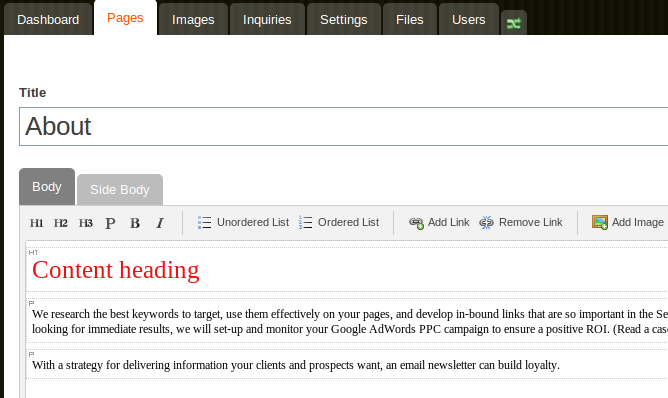
\includegraphics[scale=0.3]{images/analyse/refinery/contentsections.png}
\caption{Seitenbearbeitung in Refinery CMS mit geöffneten Content Sections Body und Site Body}
\label{contentsections}
\end{center}
\end{figure}
\item[Bilder- und Dateien-Modul]\mbox{~}\\*
In Refinery wird durch die Wahl der Menüpunkte Bilder und Dateien die Ressourcenverwaltung des Systems geöffnet. Dort können anschließend 	Mediendateien verschiedenster Formate hochgeladen, bearbeitet und durchsucht werden.
\item[Benutzer-Modul]\mbox{~}\\*
Das Benutzer-Modul erlaubt die Verwaltung der am System registrierten 	Anwender. U.a. können dort Nutzername, Passwort und Berechtigungen für die Verwendung anderer Module gesetzt werden.
\item[Einstellungs-Modul]\mbox{~}\\*
Die einzelnen Module und Erweiterungen von Refinery können durch zuvor definierte Parameter\footnote{Die offizielle Bezeichnung der Parameter lautet \emph{Refinery Settings}} in ihrem Verhalten oder Ausehen beeinflusst werden. Das Einstellungs-Modul listet die in einer CMS-Installation vorhandenen Konfigurationsoptionen auf und ermöglicht eine nachträgliche Editierung und Löschung dieser.
\end{description}
\subsection{Erweiterungen}
Erweiterungen werden in Refinery als Engines bezeichnet. Sie werden durch Aktivierung innerhalb der Rails-Anwendung (im Quellcode) installiert und anschließend im Benutzer-Modul von Refinery den einzelnen Anwendern zugeordnet. Zum Zeitpunkt der Erstellung dieser Arbeit existieren u.a. folgende Erweiterungen:
\begin{itemize}
\item
refinerycms-inquiries\footnote{Komponenten-Download: \href{https://github.com/resolve/refinerycms-inquiries}{https://github.com/resolve/refinerycms-inquiries}}: Darstellung von Kontaktanfragen auf der Internetseite mit zusätzlicher Verwaltungsfunktion der Anfragen im Backend von Refinery CMS
\item
refinerycms-news\footnote{Komponenten-Download: \href{https://github.com/resolve/refinerycms-news}{https://github.com/resolve/refinerycms-news}}: Verwaltung und Darstellung von Nachrichten im Front- und Backend-Bereich
\item
 refinerycms-blog\footnote{Komponenten-Download: \href{https://github.com/resolve/refinerycms-blog}{https://github.com/resolve/refinerycms-blog}}: Engine zur Erstellung kurzer Beiträge inklusive Kategorisierungs- und Kommentarfunktion
\end{itemize}

\subsection{Verwendete Technologien}
Refinery CMS ist ein technologisch sehr einfaches System. Die Realisierung der Backend-Funktionalitäten wird durch die konsequente Verwendung von HTML 5 erreicht. Zur Generierung der Dialoge, die u.a. innerhalb des Bild- und Dateien-Moduls eingesetzt werden, greift Refinery auf die jQuery UI Bibliothek zurück. Der im Seiten-Modul integrierte WYSIWYG-Editor ist ein für die Anforderungen des CMS angepasster, XHTML konformer JavaScript WYMeditor.
Durch die Unterstützung von HTML 5 innerhalb des Backend können Datenübertragungen von Medien an den Server in Form von Multi-Uploads realisiert werden. Die sonst übliche Nutzung von Flash entfällt und vereinfacht damit das System zusätzlich.
Die bereits angesprochenen Erweiterungen (Engines) sind eigenständige Rails-Anwendungen, deren Grundgerüst mit Hilfe eines Refinery-Engine-Generators erzeugt wird.
Die geringen technologischen Abhängigkeiten und Anforderungen des Systems erlauben es, Teile des Backends bei Bedarf anzupassen, zu verändern oder komplett auszutauschen.
%Refinery END


\section{Durchführung der funktionalen Analyse}
\label{sec:durchanalyse}
Um die Leistungsfähigkeit der ausgewählten Systeme im Bereich des Webpublishing einschätzen zu können, werden die vorgestellten Kriterien des vorhergehenden Abschnitts mit den ausgewählten WCMS in Tabellenform gegenübergestellt. Es erfolgt dabei eine Festlegung der Erfüllung dieser Kriterien in folgende 2 Stufen:

\begin{table}[!h]
\renewcommand{\arraystretch}{1.5}
\center
\caption{Mögliche Auswertungsstufen für die umgesetzten Funktionalitäten der WCMS}
\begin{tabular}{|l|p{10cm}|}
\hline
\cellcolor{green} Erfüllt 100\% & Das hier vorgestellte WCMS erfüllt die aus dem
Kriterium definierten Funktionalitäten. Dies kann auch durch Installation einer Zusatzkomponente erreicht werden.\\
\hline
\cellcolor{red} Erfüllt 0\% & Das hier vorgestellte WCMS erfüllt die aus dem
Kriterium definierten Funktionalitäten nicht. Es existieren darüber hinaus keine Erweiterungsmöglichkeiten für das System oder die Erfüllung ist nur durch eigenständige Implementierung (Programmierung) erreichbar.\\
\hline
\end{tabular}
\end{table}
Zusätzlich werden bei bestehenden Einschränkungen und Problemen zu jedem WCMS noch Erläuterungen aufgeführt, die eine genauere Einschätzung des tatsächlichen Funktionsumfangs liefern können.
\subsection{Erstellung}
\begin{tabular}[!ht]{|l|l|l|l|}
\hline
\multicolumn{4}{|p{15cm}|}{\textbf{Mehrere Benutzer sollen gleichzeitig Inhalte verwalten und erfassen können}} \\
\hline
  Alchemy 1.6.0 & \cellcolor{green}Erfüllt: 100\% & Refinery CMS 1.0.8 & \cellcolor{green}Erfüllt: 100\% \\
  \hline
  \multicolumn{2}{|p{7.5cm}|}{Nutzer und Administratoren können Inhalte gleichzeitig erfassen und verwalten.}
   & \multicolumn{2}{p{7.5cm}|}{Nutzer und Administratoren können Inhalte gleichzeitig erfassen und verwalten.} \\
  \hline
  Browser CMS 3.3.1 & \cellcolor{green}Erfüllt: 100\% & Locomotive CMS & \cellcolor{green}Erfüllt: 100\% \\
  \hline
  \multicolumn{2}{|p{7.5cm}|}{Nutzer und Administratoren können Inhalte gleichzeitig erfassen und verwalten.} & \multicolumn{2}{p{7.5cm}|}{Nutzer und Administratoren können Inhalte gleichzeitig erfassen und verwalten.} \\
\hline
\end{tabular}
\newline
\newline
\newline
\begin{tabular}[!ht]{|l|l|l|l|}
\hline
\multicolumn{4}{|p{15cm}|}{\textbf{Inhalte sollen – unabhängig von Zeit- und Standort – durch mehrere Benutzer online verwaltet und erfasst werden können}} \\
\hline
  Alchemy 1.6.0 & \cellcolor{green}Erfüllt: 100\% & Refinery CMS 1.0.8 & \cellcolor{green}Erfüllt: 100\% \\
  \hline
  \multicolumn{2}{|p{7.5cm}|}{Vollständig unterstützt} & \multicolumn{2}{p{7.5cm}|}{Vollständig unterstützt} \\
  \hline
  Browser CMS 3.3.1 & \cellcolor{green}Erfüllt: 100\% & Locomotive CMS & \cellcolor{green}Erfüllt: 100\% \\
  \hline
  \multicolumn{2}{|p{7.5cm}|}{Vollständig unterstützt} & \multicolumn{2}{p{7.5cm}|}{Vollständig unterstützt} \\
\hline
\end{tabular}
\newline
\newline
\newline
\begin{tabular}[!ht]{|l|l|l|l|}
\hline
\multicolumn{4}{|p{15cm}|}{\textbf{Offline Erfassung von Inhalten unter Verwendung eines lokal auf dem Rechner installierten Programms}} \\
\hline
  Alchemy 1.6.0 & \cellcolor{red}Erfüllt: 0\% & Refinery CMS 1.0.8 & \cellcolor{red}Erfüllt: 0\% \\
  \hline
  \multicolumn{2}{|p{7.5cm}|}{Wird nicht unterstützt} & \multicolumn{2}{p{7.5cm}|}{Wird nicht unterstützt} \\
  \hline
  Browser CMS 3.3.1 & \cellcolor{red}Erfüllt: 0\% & Locomotive CMS & \cellcolor{red}Erfüllt: 0\% \\
  \hline
  \multicolumn{2}{|p{7.5cm}|}{Wird nicht unterstützt} & \multicolumn{2}{p{7.5cm}|}{Wird nicht unterstützt} \\
\hline
\end{tabular}
\newline
\newline
\newline
\begin{tabular}[!ht]{|l|l|l|l|}
\hline
\multicolumn{4}{|p{15cm}|}{\textbf{Integrierte Mediendatenbank zur Erfassung und Verwaltung von Bildern, Multimedia,Texten, Audio, Videos, usw.}} \\
\hline
  Alchemy 1.6.0 & \cellcolor{green}Erfüllt: 100\% & Refinery CMS 1.0.8 & \cellcolor{green}Erfüllt: 100\% \\
  \hline
  \multicolumn{2}{|p{7.5cm}|}{Alchemy bietet eine Bibliothek, in der Bilder und Dateien verwaltet werden können.}
   & \multicolumn{2}{p{7.5cm}|}{Refinery CMS bietet eine einfache Medienverwaltung.} \\
  \hline
  Browser CMS 3.3.1 & \cellcolor{green}Erfüllt: 100\% & Locomotive CMS & \cellcolor{green}Erfüllt: 100\% \\
  \hline
  \multicolumn{2}{|p{7.5cm}|}{Browser CMS verfügt über eine \emph {Content Library}, die eine einfache Medienverwaltung von Bildern, Dateien und definierten Inhaltselementen ermöglicht.} & \multicolumn{2}{p{7.5cm}|}{Locomotive CMS bietet eine Asset-Verwaltung, in der selbst erstellte Inhaltselemente in Containern verwaltet werden können.} \\
\hline
\end{tabular}
\newline
\newline
\newline
\begin{tabular}[!ht]{|l|l|l|l|}
\hline
\multicolumn{4}{|p{15cm}|}{\textbf{Inhalte sollen ohne spezielle Programmier / HTML-Kenntnisse erfasst und verwaltet werden können}} \\
\hline
  Alchemy 1.6.0 & \cellcolor{green}Erfüllt: 100\% & Refinery CMS 1.0.8 & \cellcolor{green}Erfüllt: 100\% \\
  \hline
  \multicolumn{2}{|p{7.5cm}|}{Alle Inhalte können über den TinyMCE-Javascript WYSIWYG Editor erfasst und formatiert werden.}
   & \multicolumn{2}{p{7.5cm}|}{Alle Inhalte können über den integrierten WYSIWYG-Editor Wymeditor erfasst und formatiert werden. Der Editor ist fest in das System integriert und kann nicht ausgetauscht werden. Ein Plugin, dass die Verwendung eines anderen Editors ermöglicht ist bereits in Planung.} \\
  \hline
  Browser CMS 3.3.1 & \cellcolor{green}Erfüllt: 100\% & Locomotive CMS & \cellcolor{green}Erfüllt: 100\% \\
  \hline
  \multicolumn{2}{|p{7.5cm}|}{In Browser CMS findet der WYSIWIG-FCKEditor Verwendung. Zusätzlich stehen verschiedene Module zur Verfügung, die einen Austausch des Editors gegen andere Lösungen ermöglichen.} & \multicolumn{2}{p{7.5cm}|}{Alle Inhalte können über zwei integrierte WYSIWYG-Editoren erfasst und formatiert werden. Im Backend steht der Javascript Editor TinyMCE zur Verfügung. Im Frontend findet der HTML5-WYSIWYG-Editor Aloha zur Manipulierung der Seiteninhalte Verwendung (befindet sich noch in der Entwicklung).} \\
\hline
\end{tabular}
\newline
\newline
\newline
\begin{tabular}[!ht]{|l|l|l|l|}
\hline
\multicolumn{4}{|p{15cm}|}{\textbf{Inhalte sollen in einer Datenbank gespeichert werden}} \\
\hline
  Alchemy 1.6.0 & \cellcolor{green}Erfüllt: 100\% & Refinery CMS 1.0.8 & \cellcolor{green}Erfüllt: 100\% \\
  \hline
  \multicolumn{2}{|p{7.5cm}|}{Alchemy verwendet Active Record als Datenbankpersistenzschicht. Durch die Verwendung von Migrationen könen so eine Vielzahl relationaler Datenbanken unterstützt werden. Zusätzlich exisitieren einige Adapter, um auch dokumentenbasierte Datenbanken anzusteuern.}
   & \multicolumn{2}{p{7.5cm}|}{Refinery greift ebenfalls auf Rails' Active Record zurück und unterstützt damit mehrere relationale und dokumentenorientierte Datenbanken.} \\
  \hline
  Browser CMS 3.3.1 & \cellcolor{green}Erfüllt: 100\% & Locomotive CMS & \cellcolor{green}Erfüllt: 100\% \\
  \hline
  \multicolumn{2}{|p{7.5cm}|}{Wie bei Alchemy und Refinery CMS wird hier auch auf Active Record zurückgegriffen. Die Entwickler garantieren auf Grund fehlender Tests jedoch nur die Unterstützung von SQLite und MySQL-Datenbanken. Tendenziell können aber alle von Active Record unterstützten Datenbanken eingesetzt werden.} & \multicolumn{2}{p{7.5cm}|}{Locomotive CMS greift im Gegensatz zu seinen Konkurrenten auf die dokumentenorientierten Datenbank MongoDB zurück. Relationale Datenbanken werden somit nicht unterstützt. Eine Umsetzung von Locomotive mit Active Record ist jedoch geplant.} \\
\hline
\end{tabular}
\newline
\newline
\newline
\begin{tabular}[!ht]{|l|l|l|l|}
\hline
\multicolumn{4}{|p{15cm}|}{\textbf{Inhalte (Texte, Bilder, Videos etc.) sollen zentral kategorisiert, erfasst und verwaltet werden können}} \\
\hline
  Alchemy 1.6.0 & \cellcolor{red}Erfüllt: 0\% & Refinery CMS 1.0.8 & \cellcolor{red}Erfüllt: 0\% \\
  \hline
  \multicolumn{2}{|p{7.5cm}|}{Die Bibliothek von Alchemy unterstützt lediglich eine Auflistung von Resourcen. Bilder und Dateien können damit nur in Form einer Listenansicht inspiziert werden. Eine Zuordnung zu Kategorien oder eine Anlage von Ordnerstrukturen zur Erleichterung der Orientierung ist nicht möglich. Die Verwaltung großer Datenmengen scheint daher nur schwer möglich.}
   & \multicolumn{2}{p{7.5cm}|}{Ähnlich wie bei Alchemy gleicht die Resourcenverwaltung nur einer einfachen Auflistung von Bildern und anderen Ressourcen. Eine Kategorisierung der Inhalte ist nicht möglich. Ebenfalls können keine Ordner zur sinnvollen Strukturierung der Ressourcen erstellt werden. Die Verwaltung großer Datenmengen wird dadurch schnell zu einem Geduldsakt.} \\
  \hline
  Browser CMS 3.3.1 & \cellcolor{red}Erfüllt: 0\% & Locomotive CMS & \cellcolor{red}Erfüllt: 0\% \\
  \hline
  \multicolumn{2}{|p{7.5cm}|}{Die \emph{Content Library} von Browser CMS listet wie ihre Vorgänger lediglich die angelegten Bilder oder Dateien auf. Möglichkeiten zur sinnvollen Organisation (Kategorien, Ordner) großer Datenmengen sind nicht vorhanden.} & \multicolumn{2}{p{7.5cm}|}{Die Inhaltsverwaltung kann nicht kategorisiert werden. Wie bei seinen Vorgängern sind die Datensätze lediglich in Listenform aufgeführt. Eine logische Strukturierung mit Hilfe von Ordnern ist nicht möglich.} \\
\hline
\end{tabular}
\newline
\newline
\newline
\begin{tabular}[!ht]{|l|l|l|l|}
\hline
\multicolumn{4}{|p{15cm}|}{\textbf{Inhalte können während der Erfassung über eine Preview-Funktion vorab im Design der Webseite angesehen werden}} \\
\hline
  Alchemy 1.6.0 & \cellcolor{green}Erfüllt: 100\% & Refinery CMS 1.0.8 & \cellcolor{red}Erfüllt: 0\% \\
  \hline
  \multicolumn{2}{|p{7.5cm}|}{Redakteure können ihre erstellten und editierten Inhalte im Backend durch ein Preview-Fenster sichtbar machen. Änderungen an Inhaltselementen können somit sofort nachvollzogen werden.}
   & \multicolumn{2}{p{7.5cm}|}{Refinery CMS verfügt über keine Preview-Funktion der Inhalte. Ist ein Inhaltselement im Backend neu angelegt oder bearbeitet wurden, wird dies auf der Internetseite sofort sichtbar.} \\
  \hline
  Browser CMS 3.3.1 & \cellcolor{green}Erfüllt: 100\% & Locomotive CMS & \cellcolor{red}Erfüllt: 0\% \\
  \hline
  \multicolumn{2}{|p{7.5cm}|}{Wie bei Alchemy werden Inhalte erst nach ihrer Veröffentlichung sichtbar. Bis dahin kann jedoch im Frontend durch Inline-Editing der Seite jedes Inhaltselement bearbeitet werden.} & \multicolumn{2}{p{7.5cm}|}{Locomotive CMS bietet wie RefineryCMS keine Preview-Funktion. Änderungen und neu angelegte Inhalte werden direkt veröffentlicht.} \\
\hline
\end{tabular}
\newline
\newline
\newline
\begin{tabular}[!ht]{|l|l|l|l|}
\hline
\multicolumn{4}{|p{15cm}|}{\textbf{Zuordnung von standardisierten und frei definierbaren Metadaten zu Inhalten (z.B. Autor, Schlüsselwörter, Benutzerdefinierte Felder) soll möglich sein}} \\
\hline
  Alchemy 1.6.0 & \cellcolor{red}Erfüllt: 0\% & Refinery CMS 1.0.8 & \cellcolor{red}Erfüllt: 0\% \\
  \hline
  \multicolumn{2}{|p{7.5cm}|}{Metadaten zu Inhalten können nicht vergeben werden.}
   & \multicolumn{2}{p{7.5cm}|}{Inhalte werden als einfache Datensätze betrachtet und besitzen daher keine definierten Metadaten.} \\
  \hline
  Browser CMS 3.3.1 & \cellcolor{green}Erfüllt: 100\% & Locomotive CMS & \cellcolor{green}Erfüllt: 100\% \\
  \hline
  \multicolumn{2}{|p{7.5cm}|}{Metadaten können zu einzelnen Inhaltselementen in Form einer Tag-Liste hinzugefügt werden. Diese wird in der Datenbank als Text abgespeichert und bei ihrer Nutzung in einzelne Teil-Strings zerlegt. Das Hinzufügen zuvor definierter Metadaten ist nicht möglich.} & \multicolumn{2}{p{7.5cm}|}{Zu den verschiedenen Inhaltselementen können beliebig viele Metadaten hinzugefügt werden. Auch die Darstellung von 1:1 und 1:n-Beziehungen ist möglich. Diese Funktionalität wird dabei vor allem durch die Verwendung der dokumentenbasierten Datenbank MongoDB möglich.} \\
\hline
\end{tabular}
\newline
\newline
\newline
\begin{tabular}[!ht]{|l|l|l|l|}
\hline
\multicolumn{4}{|p{15cm}|}{\textbf{Inhalte sollen mehrsprachig erfasst und verwaltet werden können}} \\
\hline
  Alchemy 1.6.0 & \cellcolor{green}Erfüllt: 100\% & Refinery CMS 1.0.8 & \cellcolor{green}Erfüllt: 100\% \\
  \hline
  \multicolumn{2}{|p{7.5cm}|}{In Alchemy können Inhalte mehrsprachig angelegt werden. Durch die Auswahl einer bestimmten Sprache wird ein entsprechender Seitenbaum mit allen existierenden Inhalten zu der ausgewählten Sprache erzeugt.}
   & \multicolumn{2}{p{7.5cm}|}{Refinery CMS kann Inhalte mehrsprachig verwalten und ausgeben. Zur Aktivierung der Funktionalität müssen nur die zu unterstützenden Sprachen in einer Konfigurationsdatei angegeben werden (dies kann von Administtratoren im Backend vorgenommen werden). Alle Sprachen werden dabei in einem einzigen Seitenbaum verwaltet. Vorhandene Übersetzungen zu einer bestimmten Seite werden durch Einblendung von Flaggensymbolen kenntlich gemacht.} \\
  \hline
  Browser CMS 3.3.1 & \cellcolor{red}Erfüllt: 0\% & Locomotive CMS & \cellcolor{red}Erfüllt: 0\% \\
  \hline
  \multicolumn{2}{|p{7.5cm}|}{In Browser CMS kann  durch die Installation der Erweiterung \emph{browsercmsi} die Unterstützung von mehrsprachigen Inhalten erreicht werden. Der Plugin-Anbieter konnte die 100\% Rails 3-Kompatibilität der Erweiterung jedoch nicht garantieren. Von einem Einsatz dieser Lösung in einer Produktiv-Umgebung wird daher abgeraten. Innerhalb der Bewertung von Browser CMS werden daher 0\% beim Erfüllungsgrad angegeben.} & \multicolumn{2}{p{7.5cm}|}{Inhalte können nur einsprachig verwaltet werden. Erweiterungen, die diese Funktionalität herstellen können, konnten nicht ermittelt werden.} \\
\hline
\end{tabular}
\newline
\newline
\newline
\begin{tabular}[!ht]{|l|l|l|l|}
\hline
\multicolumn{4}{|p{15cm}|}{\textbf{Das CMS soll über eine offene API (Programmierschnittstelle) für individuelle Erweiterung verfügen}} \\
\hline
  Alchemy 1.6.0 & \cellcolor{green}Erfüllt: 100\% & Refinery CMS 1.0.8 & \cellcolor{green}Erfüllt: 100\% \\
  \hline
  \multicolumn{2}{|p{7.5cm}|}{Eine flexible Plugin-DSL (Domain Specific Language) erlaubt das Hinzufügen von individuellen Erweiterungen.}
   & \multicolumn{2}{p{7.5cm}|}{Individuelle Inhaltselemente können durch die Verwendung der Refinery Engine Generatoren hinzugefügt werden. Die weitere Entwicklung Anpassung des Codegerüst folgt dann mit den inenrhalb des Rails Framework üblichen Entwicklungstechniken und -abläufen.} \\
  \hline
  Browser CMS 3.3.1 & \cellcolor{green}Erfüllt: 100\% & Locomotive CMS & \cellcolor{green}Erfüllt: 100\% \\
  \hline
  \multicolumn{2}{|p{7.5cm}|}{Ähnlich wie bei Refinery CMS können neue Module und Inhaltstypen mit Hilfe von speziellen Rails-Generatoren erzeugt werden.} & \multicolumn{2}{p{7.5cm}|}{Neue Inhaltstypen lassen sich im Backend durch ein einfaches User-Interface zusammenstellen.  Mit wenigen Klicks sind so schnell neue Elemente erstellt. Programmierkenntnisse sind nicht notwendig.} \\
\hline
\end{tabular}
\newline
\newline
\newline
\begin{tabular}[!ht]{|l|l|l|l|}
\hline
\multicolumn{4}{|p{15cm}|}{\textbf{Für die Verwaltung und Erfassung von Inhalten sollen alle gängigen Internet-Browser (Internet Explorer, Safari und Firefox) eingesetzt werden können}} \\
\hline
  Alchemy 1.6.0 & \cellcolor{green}Erfüllt: 100\% & Refinery CMS 1.0.8 & \cellcolor{green}Erfüllt: 100\% \\
  \hline
  \multicolumn{2}{|p{7.5cm}|}{Vollständig unterstützt}
   & \multicolumn{2}{p{7.5cm}|}{Vollständig unterstützt} \\
  \hline
  Browser CMS 3.3.1 & \cellcolor{green}Erfüllt: 100\% & Locomotive CMS & \cellcolor{green}Erfüllt: 100\% \\
  \hline
  \multicolumn{2}{|p{7.5cm}|}{Vollständig unterstützt} & \multicolumn{2}{p{7.5cm}|}{Vollständig unterstützt} \\
\hline
\end{tabular}
\newline
\newline
\newline
\begin{tabular}[!ht]{|l|l|l|l|}
\hline
\multicolumn{4}{|p{15cm}|}{\textbf{Inhalte sollen einfach importiert / exportiert werden können - dabei kommen Formate wie z.B. XML zum Einsatz}} \\
\hline
  Alchemy 1.6.0 & \cellcolor{red}Erfüllt: 0\% & Refinery CMS 1.0.8 & \cellcolor{red}Erfüllt: 0\% \\
  \hline
  \multicolumn{2}{|p{7.5cm}|}{Alchemy verfügt über keine integrierten Import und Export-Funktionalitäten.}
   & \multicolumn{2}{p{7.5cm}|}{Es existieren auf Nutzerebene keine Möglichkeiten des Im- und Exports. Durch sogenannte Seed-Dateien ist jedoch ein nachträgliches Befüllen der Datenbank möglich. Der Aufruf erfordert jedoch Kenntnisse in Ruby on Rails und ist daher für Normalanwender/Redakteure nicht sinnvoll.} \\
  \hline
  Browser CMS 3.3.1 & \cellcolor{red}Erfüllt: 0\% & Locomotive CMS & \cellcolor{green}Erfüllt: 100\% \\
  \hline
  \multicolumn{2}{|p{7.5cm}|}{In Browser CMS können Inhalte nicht importiert und exportiert werden. Entsprechende Features müssten erst eigenständig implementiert werden.} & \multicolumn{2}{p{7.5cm}|}{In Locomotive CMS kann ein kompletter Internetauftritt mit seinen Inhalten und Ressourcen importiert und exportiert werden. Zum Austausch der Inhalte findet eine \emph{Zip}-Datei Verwendung, die alle benötigten Ressourcen (Bilder, Dateien, Templates usw.) sowie Inhalte der Datenbank einschließt. Ressourcen werden dabei in vordefinierten Ordnerstrukturen abgelegt. Die Datenbankeinträge aus MongoDB werden innerhalb der \emph{Zip}-Datei im Unterordner \emph{data} abgelegt. Die Einträge liegen dabei  im \emph{YAML}-Format vor.} \\
\hline
\end{tabular}
\newline
\newline
\newline
\begin{tabular}[!ht]{|l|l|l|l|}
\hline
\multicolumn{4}{|p{15cm}|}{\textbf{Integration von Inhalten anderer Webseiten, Multimedia, Applikationen, E-Commerce-Tools}} \\
\hline
  Alchemy 1.6.0 & \cellcolor{green}Erfüllt: 100\% & Refinery CMS 1.0.8 & \cellcolor{green}Erfüllt: 100\% \\
  \hline
  \multicolumn{2}{|p{7.5cm}|}{Der verwendete WYSIWYG-Editor \emph{TinyMCE} erlaubt in seiner HTML-Ansicht das Einbinden von Fremdinhalten anderer Seiten (z.B. IFrame). Zusätzlich ist die Erstellung von eigenen Inhaltselementen mit Hilfe der Alchemy Plugin DSL-API denkbar. So können auch die verschiedenen Resourcen aus der Bibliothek von Alchemy Verwendung finden. Standardmäßig verfügt Alchemy bereits über die Inhaltselemente \emph{Artikel}, \emph{Text}, \emph{Text mit Bild}, \emph{Bilder}, \emph{Bildergalerie}, \emph{Überschrift} und \emph{Intro}.}
   & \multicolumn{2}{p{7.5cm}|}{Refinery CMS verwaltet jede Internetseite innerhalb eines flexiblen WYSIWYG-Editors. Die Integration von vordefiniertem HTML-Code kann dabei durch Nutzung der HTML-Ansicht des Editors erreicht werden.
} \\
  \hline
  Browser CMS 3.3.1 & \cellcolor{green}Erfüllt: 100\% & Locomotive CMS & \cellcolor{green}Erfüllt: 100\% \\
  \hline
  \multicolumn{2}{|p{7.5cm}|}{Wie seine Vorgänger auch können innerhalb des WYSIWYG-Editors IFrames oder anderer HTML-Code eingebetet werden. Vordefinierte Inhaltselemente, die vorhandene Ressourcen aus der \emph{Content Library} einbinden können, müssen eigenhändig angelegt werden.} & \multicolumn{2}{p{7.5cm}|}{Wie bei Alchemy und Refinery CMS können innerhalb des  WYSIWYG-Editors HTML-Fragmente angegeben werden.} \\
\hline
\end{tabular}
\subsection{Kontrolle}
\begin{tabular}[!ht]{|l|l|l|l|}
\hline
\multicolumn{4}{|p{15cm}|}{\textbf{Granulares Rechte- und Rollenkonzept für Anwender}} \\
\hline
  Alchemy 1.6.0 & \cellcolor{red}Erfüllt: 0\% & Refinery CMS 1.0.8 & \cellcolor{red}Erfüllt: 0\% \\
  \hline
  \multicolumn{2}{|p{7.5cm}|}{In Alchemy existieren vordefinierte Rollen (Registriert, Author, Redakteur,Administrator). Das Anlegen weiterer Rollen zur besseren Differenzierung ist jedoch nicht möglich.}
   & \multicolumn{2}{p{7.5cm}|}{Refinery CMS besitzt kein Rechte- und Rollenkonzept. Dem Anwender kann lediglich der Zugang zu bestimmten Plugins erlaubt oder entzogen werden, um so den Funktionsumfang einzuschränken.} \\
  \hline
  Browser CMS 3.3.1 & \cellcolor{green}Erfüllt: 100\% & Locomotive CMS & \cellcolor{red}Erfüllt: 0\% \\
  \hline
  \multicolumn{2}{|p{7.5cm}|}{In Browser CMS wird in einer Standardinstallation zwischen den Rollen Gast, CMS Administrator und Content Editor unterschieden. Zusätzlich können weitere Backend-Gruppen angelegt werden.} & \multicolumn{2}{p{7.5cm}|}{Locomotive CMS besitzt ein einfaches Rechte- und Rollenkonzept. Es wird zwischen Administratoren, Designern und Autoren unterschieden. Das Anlegen weiterer Gruppen ist nicht möglich.} \\
\hline
\end{tabular}
\newline
\newline
\newline
\begin{tabular}[!ht]{|l|l|l|l|}
\hline
\multicolumn{4}{|p{15cm}|}{\textbf{Granulares Berechtigungskonzept für einzelne Inhalte, Bereiche, Webseiten}} \\
\hline
  Alchemy 1.6.0 & \cellcolor{red}Erfüllt: 0\% & Refinery CMS 1.0.8 & \cellcolor{red}Erfüllt: 0\% \\
  \hline
  \multicolumn{2}{|p{7.5cm}|}{Die in Alchemy vordefinierte Rollen Registriert, Author, Redakteur und Administrator bestimmen den Funktionsumfang eines Anwenders im Backend. Angelegte Inhalte können jedoch nicht einzelnen Nutzern zugeordnet werden.}
   & \multicolumn{2}{p{7.5cm}|}{Nutzer können alle Inhalte und Bereiche einer Webseite editieren, solange sie zur Nutzung des bestimmten Plugins berechtigt wurden.} \\
  \hline
  Browser CMS 3.3.1 & \cellcolor{red}Erfüllt: 0\% & Locomotive CMS & \cellcolor{red}Erfüllt: 0\% \\
  \hline
  \multicolumn{2}{|p{7.5cm}|}{ Der Zugriff auf bestimmte Seiten (Seitenbaumzweige)  kann eingeschränkt werden. Zusätzlich bietet Browser CMS ein Erstellen von Frontend-Nutzergruppen an, um so bestimmte Seiten des CMS nur exklusiv ausgewählten Nutzern zur Verfügung zu stellen. Die Zugriffsberechtigung auf installierte Plugins kann ebenfalls für jeden Nutzer individuell festgelegt werden. Leider ist es nicht möglich, einzelne Inhaltselemente für bestimmte Nutzer unzugänglich zu machen.} & \multicolumn{2}{p{7.5cm}|}{Der Zugriff auf Seiten und Inhalte kann nicht individuell gesteuert und beeinflusst werden. Besitzt ein Anwender das Recht zum Editieren und Anlegen von Inhalten (Nutzergruppe Redakteur), können alle Inhalte im gesamten CMS bearbeitet werden.} \\
\hline
\end{tabular}
\newline
\newline
\newline
\begin{tabular}[!ht]{|l|l|l|l|}
\hline
\multicolumn{4}{|p{15cm}|}{\textbf{Schutz vor gegenseitigem Überschreiben erfasster Inhalte durch Check in/ Check out-Mechanismen}} \\
\hline
  Alchemy 1.6.0 & \cellcolor{red}Erfüllt: 0\% & Refinery CMS 1.0.8 & \cellcolor{red}Erfüllt: 0\% \\
  \hline
  \multicolumn{2}{|p{7.5cm}|}{Wird nicht unterstützt} & \multicolumn{2}{p{7.5cm}|}{Wird nicht unterstützt} \\
  \hline
  Browser CMS 3.3.1 & \cellcolor{red}Erfüllt: 0\% & Locomotive CMS & \cellcolor{red}Erfüllt: 0\% \\
  \hline
  \multicolumn{2}{|p{7.5cm}|}{Wird nicht unterstützt. Die automatische Versionierung von Inhaltselementen erlaubt jedoch ein nachträgliches, manuelles Sichten und Zusammenfügen  verschiedener Versionen.} & \multicolumn{2}{p{7.5cm}|}{Wird nicht unterstützt} \\
\hline
\end{tabular}
\newline
\newline
\newline
\begin{tabular}[!ht]{|l|l|l|l|}
\hline
\multicolumn{4}{|p{15cm}|}{\textbf{Versionierung von Inhalten mit Möglichkeit zur Wiederherstellung vorhergehender Versionen}} \\
\hline
  Alchemy 1.6.0 & \cellcolor{red}Erfüllt: 0\% & Refinery CMS 1.0.8 & \cellcolor{red}Erfüllt: 0\% \\
  \hline
  \multicolumn{2}{|p{7.5cm}|}{Versionierung und Wiederherstellung von Inhalten wird nicht unterstüzt.} & \multicolumn{2}{p{7.5cm}|}{Versionierung und Wiederherstellung von Inhalten wird nicht unterstüzt.} \\
  \hline
  Browser CMS 3.3.1 & \cellcolor{green}Erfüllt: 100\% & Locomotive CMS & \cellcolor{red}Erfüllt: 0\% \\
  \hline
  \multicolumn{2}{|p{7.5cm}|}{Wird unterstützt} & \multicolumn{2}{p{7.5cm}|}{Versionierung und Wiederherstellung von Inhalten wird nicht unterstüzt.} \\
\hline
\end{tabular}
\newline
\newline
\newline
\begin{tabular}[!ht]{|l|l|l|l|}
\hline
\multicolumn{4}{|p{15cm}|}{\textbf{Mandantenfähigkeit: Mehrfachnutzung des Systems durch verschiedene Parteien mit kompletter Trennung der Daten und Benutzer}} \\
\hline
  Alchemy 1.6.0 & \cellcolor{red}Erfüllt: 0\% & Refinery CMS 1.0.8 & \cellcolor{red}Erfüllt: 0\% \\
  \hline
  \multicolumn{2}{|p{7.5cm}|}{Wird nicht unterstüzt} & \multicolumn{2}{p{7.5cm}|}{Wird nicht unterstüzt} \\
  \hline
  Browser CMS 3.3.1 & \cellcolor{red}Erfüllt: 0\% & Locomotive CMS & \cellcolor{red}Erfüllt: 0\% \\
  \hline
  \multicolumn{2}{|p{7.5cm}|}{Wird nicht unterstüzt} & \multicolumn{2}{p{7.5cm}|}{In Locomotive CMS können mehrere Internetauftritte gleichzeitig verwaltet werden. Eine Trennung der verschiedenen Nutzer und Daten wird jedoch nicht angeboten.} \\
\hline
\end{tabular}
\newline
\newline
\newline
\begin{tabular}[!ht]{|l|l|l|l|}
\hline
\multicolumn{4}{|p{15cm}|}{\textbf{Linküberprüfung: Automatische Prüfung der Gültigkeit von internen und externen Links mit Möglichkeit zur Korrektur bzw. Benachrichtigung definierter Personengruppen}} \\
\hline
  Alchemy 1.6.0 & \cellcolor{red}Erfüllt: 0\% & Refinery CMS 1.0.8 & \cellcolor{red}Erfüllt: 0\% \\
  \hline
  \multicolumn{2}{|p{7.5cm}|}{Wird nicht unterstüzt} & \multicolumn{2}{p{7.5cm}|}{Wird nicht unterstüzt} \\
  \hline
  Browser CMS 3.3.1 & \cellcolor{red}Erfüllt: 0\% & Locomotive CMS & \cellcolor{red}Erfüllt: 0\% \\
  \hline
  \multicolumn{2}{|p{7.5cm}|}{Wird nicht unterstüzt} & \multicolumn{2}{p{7.5cm}|}{Wird nicht unterstüzt} \\
\hline
\end{tabular}


\subsection{Freigabe}
\begin{tabular}[!ht]{|l|l|l|l|}
\hline
\multicolumn{4}{|p{15cm}|}{\textbf{Möglichkeit für \emph{nicht technische} User den Workflow zu kreieren, verwalten und zu ändern. Es soll dafür kein Scripting / Programming notwendig sein}} \\
\hline
  Alchemy 1.6.0 & \cellcolor{red}Erfüllt: 0\% & Refinery CMS 1.0.8 & \cellcolor{red}Erfüllt: 0\% \\
  \hline
  \multicolumn{2}{|p{7.5cm}|}{Nutzer können in Alchemy keinen Workflowprozess kreieren. Es ist jedoch möglich, das Redakteure die von Autoren durchgeführten Änderungen kontrollieren und anschließend veröffentlichen.
Ein Austausch zwischen beiden Nutzergruppen ist nicht möglich (z.B. kurze Mitteilung an den Redakteur). Redakteure müssen so Änderungen der Seiteninhalte selbst erkennen.} & \multicolumn{2}{p{7.5cm}|}{Wird nicht unterstüzt} \\
  \hline
  Browser CMS 3.3.1 & \cellcolor{red}Erfüllt: 0\% & Locomotive CMS & \cellcolor{red}Erfüllt: 0\% \\
  \hline
  \multicolumn{2}{|p{7.5cm}|}{Ein Workflowprozess kann in Browser CMS nicht erzeugt werden. Autoren ist es nur möglich, ihre durchgeführten Änderungen an andere Backend-Nutzer mit Veröffentlichungsrechten weiterzuleiten (Simulierung eines einfachsten Workflows).} & \multicolumn{2}{p{7.5cm}|}{Wird nicht unterstüzt} \\
\hline
\end{tabular}
\begin{tabular}[!ht]{|l|l|l|l|}
\hline
\multicolumn{4}{|p{15cm}|}{\textbf{Definition von Workflows inkl. mehrstufiger Freigabeprozesse für die Freischaltung von Inhalten}} \\
\hline
  Alchemy 1.6.0 & \cellcolor{red}Erfüllt: 0\% & Refinery CMS 1.0.8 & \cellcolor{red}Erfüllt: 0\% \\
  \hline
  \multicolumn{2}{|p{7.5cm}|}{Wird nicht unterstüzt} & \multicolumn{2}{p{7.5cm}|}{Wird nicht unterstüzt} \\
  \hline
  Browser CMS 3.3.1 & \cellcolor{red}Erfüllt: 0\% & Locomotive CMS & \cellcolor{red}Erfüllt: 0\% \\
  \hline
  \multicolumn{2}{|p{7.5cm}|}{Wird nicht unterstüzt} & \multicolumn{2}{p{7.5cm}|}{Wird nicht unterstüzt} \\
\hline
\end{tabular}
\newline
\newline
\newline
\begin{tabular}[!ht]{|l|l|l|l|}
\hline
\multicolumn{4}{|p{15cm}|}{\textbf{Möglichkeit externe Benutzer in Workflows mit einbinden zu können}} \\
\hline
  Alchemy 1.6.0 & \cellcolor{red}Erfüllt: 0\% & Refinery CMS 1.0.8 & \cellcolor{red}Erfüllt: 0\% \\
  \hline
  \multicolumn{2}{|p{7.5cm}|}{Wird nicht unterstützt} & \multicolumn{2}{p{7.5cm}|}{Wird nicht unterstüzt} \\
  \hline
  Browser CMS 3.3.1 & \cellcolor{red}Erfüllt: 0\% & Locomotive CMS & \cellcolor{red}Erfüllt: 0\% \\
  \hline
  \multicolumn{2}{|p{7.5cm}|}{Wird nicht unterstützt} & \multicolumn{2}{p{7.5cm}|}{Wird nicht unterstüzt} \\
\hline
\end{tabular}
\newline
\newline
\newline
\begin{tabular}[!ht]{|l|l|l|l|}
\hline
\multicolumn{4}{|p{15cm}|}{\textbf{Unternehmensspezifische Bearbeitungsprozesse von Inhalten sollen über frei definierbare Workflows verwaltet werden können}} \\
\hline
  Alchemy 1.6.0 & \cellcolor{red}Erfüllt: 0\% & Refinery CMS 1.0.8 & \cellcolor{red}Erfüllt: 0\% \\
  \hline
  \multicolumn{2}{|p{7.5cm}|}{Wird nicht unterstützt} & \multicolumn{2}{p{7.5cm}|}{Wird nicht unterstüzt} \\
  \hline
  Browser CMS 3.3.1 & \cellcolor{red}Erfüllt: 0\% & Locomotive CMS & \cellcolor{red}Erfüllt: 0\% \\
  \hline
  \multicolumn{2}{|p{7.5cm}|}{Wird nicht unterstützt} & \multicolumn{2}{p{7.5cm}|}{Wird nicht unterstüzt} \\
\hline
\end{tabular}

\subsection{Publikation}
\begin{tabular}[!ht]{|l|l|l|l|}
\hline
\multicolumn{4}{|p{15cm}|}{\textbf{Trennung von Inhalt und Design unter Verwendung von Templates}} \\
\hline
  Alchemy 1.6.0 & \cellcolor{green}Erfüllt: 100\% & Refinery CMS 1.0.8 & \cellcolor{green}Erfüllt: 100\% \\
  \hline
  \multicolumn{2}{|p{7.5cm}|}{Inhalt und Design werden in Alchemy durch die Verwendung von \emph{erb}-Templates getrennt. Das Haupt-Template der Seite wird zu Beginn der Entwicklung von einem Designer festgelegt und anschließend in der Anwendung verankert (als fixe Ressource im Rails Quellcode). So können Redakteure das Aussehen der Internetseite nicht beeinflussen.} & \multicolumn{2}{p{7.5cm}|}{Wie Alchemy verwendet Refinery CMS \emph{erb} als Template-Sprache.
Trotz der so erreichten Trennung zwischen Inhalten und Design erschwert die fehlende Möglichkeit der Anpassung im Backend den Umgang mit dem gesamten WCMS. Dies gilt für das Haupttemplate der Seite sowie für alle Erweiterungen.} \\
  \hline
  Browser CMS 3.3.1 & \cellcolor{green}Erfüllt: 100\% & Locomotive CMS & \cellcolor{green}Erfüllt: 100\% \\
  \hline
  \multicolumn{2}{|p{7.5cm}|}{Browser CMS unterstützt die Verwendung verschiedener Template-Sprachen.
In einer Standard-Installation werden u.a. \emph{erb}, \emph{rjs} und \emph{rxml} angeboten.} & \multicolumn{2}{p{7.5cm}|}{In Locomotive CMS kann für jede Seite ein Template angegeben werden. Die dabei verwendete Templatesprache ist \emph{Liquid}.} \\
\hline
\end{tabular}
\newline
\newline
\newline
\begin{tabular}[!ht]{|l|l|l|l|}
\hline
\multicolumn{4}{|p{15cm}|}{\textbf{Mehrfachverwendung von Inhalten an verschiedenen Stellen mit unterschiedlichem Layout}} \\
\hline
  Alchemy 1.6.0 & \cellcolor{green}Erfüllt: 100\% & Refinery CMS 1.0.8 & \cellcolor{red}Erfüllt: 0\% \\
  \hline
  \multicolumn{2}{|p{7.5cm}|}{Inhaltselemente und Seiten können in Alchemy kopiert und wiederverwendet werden. Die Zuordnung eines neuen Templates muss durch den Administrator erfolgen (Änderung am Rails-Quellcode).} & \multicolumn{2}{p{7.5cm}|}{Inhalte und Seiten können nicht kopiert und mehrfach verwendet werden.} \\
  \hline
  Browser CMS 3.3.1 & \cellcolor{red}Erfüllt: 0\% & Locomotive CMS & \cellcolor{red}Erfüllt: 0\% \\
  \hline
  \multicolumn{2}{|p{7.5cm}|}{Es können nur Inhalte mehrfach verwendet werden.} & \multicolumn{2}{p{7.5cm}|}{In Locomotive CMS kann nur für jede Seite ein neues Template angegeben werden. Inhalte sind den einzelnen Seiten zugeordnet und nur dort verwendbar.} \\
\hline
\end{tabular}
\newline
\newline
\newline
\begin{tabular}[!ht]{|l|l|l|l|}
\hline
\multicolumn{4}{|p{15cm}|}{\textbf{Navigationsstrukturen werden automatisch vom CMS generiert, publiziert und verwaltet}} \\
\hline
  Alchemy 1.6.0 & \cellcolor{green}Erfüllt: 100\% & Refinery CMS 1.0.8 & \cellcolor{green}Erfüllt: 100\% \\
  \hline
  \multicolumn{2}{|p{7.5cm}|}{Wird unterstützt} & \multicolumn{2}{p{7.5cm}|}{Wird unterstützt} \\
  \hline
  Browser CMS 3.3.1 & \cellcolor{green}Erfüllt: 100\% & Locomotive CMS & \cellcolor{green}Erfüllt: 100\% \\
  \hline
  \multicolumn{2}{|p{7.5cm}|}{Wird unterstützt} & \multicolumn{2}{p{7.5cm}|}{Wird unterstützt} \\
\hline
\end{tabular}
\newline
\newline
\newline
\begin{tabular}[!ht]{|l|l|l|l|}
\hline
\multicolumn{4}{|p{15cm}|}{\textbf{Barrierefreiheit bei den publizierten Seiten soll unterstützt werden}} \\
\hline
  Alchemy 1.6.0 & \cellcolor{green}Erfüllt: 100\% & Refinery CMS 1.0.8 & \cellcolor{green}Erfüllt: 100\% \\
  \hline
  \multicolumn{2}{|p{7.5cm}|}{Barrierefreiheit kann bei entsprechender Umsetzung der Verwendeten Templates und CSS-Dateien erreicht werden.} & \multicolumn{2}{p{7.5cm}|}{Barrierefreiheit kann bei entsprechender Umsetzung der Verwendeten Templates und CSS-Dateien erreicht werden.} \\
  \hline
  Browser CMS 3.3.1 & \cellcolor{green}Erfüllt: 100\% & Locomotive CMS & \cellcolor{green}Erfüllt: 100\% \\
  \hline
  \multicolumn{2}{|p{7.5cm}|}{Barrierefreiheit kann bei entsprechender Umsetzung der Verwendeten Templates und CSS-Dateien erreicht werden.} & \multicolumn{2}{p{7.5cm}|}{Barrierefreiheit kann bei entsprechender Umsetzung der Verwendeten Templates und CSS-Dateien erreicht werden.} \\
\hline
\end{tabular}
\newline
\newline
\newline
\begin{tabular}[!ht]{|l|l|l|l|}
\hline
\multicolumn{4}{|p{15cm}|}{\textbf{Inhalte sollen auf verschiedene Medien / Technologien (Cross Media Publishing, SMS /Mobile / WAP / usw.) ausgegeben werden können}} \\
\hline
  Alchemy 1.6.0 & \cellcolor{red}Erfüllt: 0\% & Refinery CMS 1.0.8 & \cellcolor{red}Erfüllt: 0\% \\
  \hline
  \multicolumn{2}{|p{7.5cm}|}{Wird nicht unterstützt} & \multicolumn{2}{p{7.5cm}|}{Wird nicht unterstützt} \\
  \hline
  Browser CMS 3.3.1 & \cellcolor{red}Erfüllt: 0\% & Locomotive CMS & \cellcolor{red}Erfüllt: 0\% \\
  \hline
  \multicolumn{2}{|p{7.5cm}|}{Wird nicht unterstützt} & \multicolumn{2}{p{7.5cm}|}{Wird nicht unterstützt} \\
\hline
\end{tabular}
\newline
\newline
\newline
\begin{tabular}[!ht]{|l|l|l|l|}
\hline
\multicolumn{4}{|p{15cm}|}{\textbf{Möglichkeit Inhalte für anderen Webseiten bereitzustellen (XML, Webservice)}} \\
\hline
  Alchemy 1.6.0 & \cellcolor{red}Erfüllt: 0\% & Refinery CMS 1.0.8 & \cellcolor{green}Erfüllt: 100\% \\
  \hline
  \multicolumn{2}{|p{7.5cm}|}{Wird nicht unterstützt} & \multicolumn{2}{p{7.5cm}|}{Es gibt Plugins mit optionaler Ausgabe als RSS-Feed oder XML. Eine Bereitstellung ausgewählter Inhalte ist damit möglich.} \\
  \hline
  Browser CMS 3.3.1 & \cellcolor{green}Erfüllt: 100\% & Locomotive CMS & \cellcolor{red}Erfüllt: 0\% \\
  \hline
  \multicolumn{2}{|p{7.5cm}|}{Die Darstellung von Inhalten als RSS-Feeds ist möglich. Es muss jedoch selbst eingerichtet werden.} & \multicolumn{2}{p{7.5cm}|}{Wird nicht unterstützt} \\
\hline
\end{tabular}
\newline
\newline
\newline
\begin{tabular}[!ht]{|l|l|l|l|}
\hline
\multicolumn{4}{|p{15cm}|}{\textbf{Möglichkeit zur Wahl zwischen dynamischer oder statischer Generierung der Seiten / Inhalte}} \\
\hline
  Alchemy 1.6.0 & \cellcolor{red}Erfüllt: 0\% & Refinery CMS 1.0.8 & \cellcolor{red}Erfüllt: 0\% \\
  \hline
  \multicolumn{2}{|p{7.5cm}|}{Wird nicht unterstützt} & \multicolumn{2}{p{7.5cm}|}{Wird nicht unterstützt} \\
  \hline
  Browser CMS 3.3.1 & \cellcolor{green}Erfüllt: 100\% & Locomotive CMS & \cellcolor{red}Erfüllt: 0\% \\
  \hline
  \multicolumn{2}{|p{7.5cm}|}{Wird unterstützt} & \multicolumn{2}{p{7.5cm}|}{Wird nicht unterstützt} \\
\hline
\end{tabular}
\newline
\newline
\newline
\begin{tabular}[!ht]{|l|l|l|l|}
\hline
\multicolumn{4}{|p{15cm}|}{\textbf{Einfache Einbindung von Fremdinhalten welche durch Drittanbieter zur Verfügung gestellt werden}} \\
\hline
  Alchemy 1.6.0 & \cellcolor{green}Erfüllt: 100\% & Refinery CMS 1.0.8 & \cellcolor{green}Erfüllt: 100\% \\
  \hline
  \multicolumn{2}{|p{7.5cm}|}{Über den integrierten WYSIWYG-Editor können HTML-Fragmente eingebunden werden.} & \multicolumn{2}{p{7.5cm}|}{Über den integrierten WYSIWYG-Editor können HTML-Fragmente eingebunden werden.} \\
  \hline
  Browser CMS 3.3.1 & \cellcolor{green}Erfüllt: 100\% & Locomotive CMS & \cellcolor{green}Erfüllt: 100\% \\
  \hline
  \multicolumn{2}{|p{7.5cm}|}{Über den integrierten WYSIWYG-Editor können HTML-Fragmente eingebunden werden.} & \multicolumn{2}{p{7.5cm}|}{Über den integrierten WYSIWYG-Editor können HTML-Fragmente eingebunden werden.} \\
\hline
\end{tabular}
\newline
\newline
\newline
\begin{tabular}[!ht]{|l|l|l|l|}
\hline
\multicolumn{4}{|p{15cm}|}{\textbf{Automatisches Anbieten von Druckversion und Weiterempfehlen einer Webseite}} \\
\hline
  Alchemy 1.6.0 & \cellcolor{red}Erfüllt: 0\% & Refinery CMS 1.0.8 & \cellcolor{red}Erfüllt: 0\% \\
  \hline
  \multicolumn{2}{|p{7.5cm}|}{Wird nicht unterstützt} & \multicolumn{2}{p{7.5cm}|}{Wird nicht unterstützt} \\
  \hline
  Browser CMS 3.3.1 & \cellcolor{red}Erfüllt: 0\% & Locomotive CMS & \cellcolor{red}Erfüllt: 0\% \\
  \hline
  \multicolumn{2}{|p{7.5cm}|}{Wird nicht unterstützt} & \multicolumn{2}{p{7.5cm}|}{Wird nicht unterstützt} \\
\hline
\end{tabular}
\subsection{Terminierung/Archivierung}
\begin{tabular}[!ht]{|l|l|l|l|}
\hline
\multicolumn{4}{|p{15cm}|}{\textbf{Freie Wahl des Publikationszeitraumes (zeitgesteuertes Auf- / Abschalten / Archivieren) von Inhalten}} \\
\hline
  Alchemy 1.6.0 & \cellcolor{red}Erfüllt: 0\% & Refinery CMS 1.0.8 & \cellcolor{red}Erfüllt: 0\% \\
  \hline
  \multicolumn{2}{|p{7.5cm}|}{Wird nicht unterstützt} & \multicolumn{2}{p{7.5cm}|}{Wird nicht unterstützt} \\
  \hline
  Browser CMS 3.3.1 & \cellcolor{red}Erfüllt: 0\% & Locomotive CMS & \cellcolor{red}Erfüllt: 0\% \\
  \hline
  \multicolumn{2}{|p{7.5cm}|}{Wird nicht unterstützt} & \multicolumn{2}{p{7.5cm}|}{Wird nicht unterstützt} \\
\hline
\end{tabular}
\newline
\newline
\newline
\begin{tabular}[!ht]{|l|l|l|l|}
\hline
\multicolumn{4}{|p{15cm}|}{\textbf{Inhalte sollen archiviert werden können.}} \\
\hline
  Alchemy 1.6.0 & \cellcolor{red}Erfüllt: 0\% & Refinery CMS 1.0.8 & \cellcolor{red}Erfüllt: 0\% \\
  \hline
  \multicolumn{2}{|p{7.5cm}|}{Wird nicht unterstützt} & \multicolumn{2}{p{7.5cm}|}{Wird nicht unterstützt} \\
  \hline
  Browser CMS 3.3.1 & \cellcolor{red}Erfüllt: 0\% & Locomotive CMS & \cellcolor{red}Erfüllt: 0\% \\
  \hline
  \multicolumn{2}{|p{7.5cm}|}{Refinery CMS erlaubt das Archivieren von kompletten Seiten. Es ist jedoch nicht möglich, bestimmte Inhalte zu Archivieren.} & \multicolumn{2}{p{7.5cm}|}{Wird nicht unterstützt} \\
\hline
\end{tabular}





\newpage
\section{Auswertung der Ergebnisse}

Der Erfüllungsgrad der einzelnen Kriterien hat für die untersuchten WCMS folgendes Gesamtergebnis herausgestellt:

\begin{table}[!h]
\renewcommand{\arraystretch}{1.5}
%\small\addtolength{\tabcolsep}{+5pt}
\center
\begin{tabular}{|l|c|c|c|c|c|}
\hline
& & \multicolumn{4}{c|}{\textbf{Web Content Management System}} \\[2pt]
\cline{3-6}
\textbf{Bereich}& \textbf{Maximum} &
\begin{sideways}
Alchemy CMS
\end{sideways}
&\begin{sideways}
Browser CMS
\end{sideways}
&\begin{sideways}
Locomotive CMS
\end{sideways}
&\begin{sideways}
Refinery CMS
\end{sideways} \\
\hline
Erstellung & 1400 & 1000 & 1000 & 1000 & 900 \\
\hline
Kontrolle & 600 & 0 & 200 & 0 & 0 \\
\hline
Freigabe & 400 & 0 & 0 & 0 & 0 \\
\hline
Publikation & 1000 & 500 & 600 & 400 & 500 \\
\hline
Terminierung/Archivierung & 200 & 0 & 0 & 0 & 0 \\
\hline
\hline
Gesamtpunkte & 3600 & 1500 & 1800 & 1400 & 1400 \\
\hline
\end{tabular}
\end{table}


Die untersuchten Systeme zeigen bei der Erfüllung der für Webpublishing relevanten Kriterien sehr unterschiedliche Resultate. Im Bereich der Inhaltserstellung vefügen die Systeme über solide Funktionalitäten. Die Webpublishingbereiche Freigabe, Kontrolle und Terminierung/Archivierung decken dagegen bei allen untersuchten Systemen funktionale Deffizite auf. In der Gesamtbetrachtung liefert Browser CMS das beste Gesamtergebnis. Vor allem durch die umfassendere Nutzer- und Rechteverwaltung kann sich das System von Alchemy CMS und Locomotive CMS absetzen, die funktional gesehen im Mittelfeld angesiedelt sind. Refinery CMS besitzt auf Grund der fehlenden Inhalts- und Rechteverwaltung die geringsten Funktionalitäten aller Systeme.
\newline
Für einen besseren Gesamtüberblick werden die Ergebnisse der durchgeführten Analyse (Kaiptel \ref{sec:durchanalyse}) für jedes System noch einmal in einer Übersicht zusammengefasst.


\subsubsection{Alchemy CMS}

\begin{description}
\item[\emph{Erstellung}]\mbox{~}\\*
\begin{itemize}
	\item Umfassende Möglichkeiten zur Erstellung und Verwaltung von Seiten und verschiedenen Inhaltselementen in verschiedenen Sprachen
	\item Template-Erstellung und -verwaltung findet im Quellcode der Rails-Anwendung statt
	\item Umsetzung komplexer Seitenlayouts möglich
\end{itemize}
\item[\emph{Kontrolle}]\mbox{~}\\*
\begin{itemize}
	\item eingeschränkte Rechteverwaltung mit festgelegten Gruppen für Front- und Backend (Registriert, Author, Redakteur, Administrator)
	\item kein umfassendes Linkmanagement
\end{itemize}
\item[\emph{Freigabe}]\mbox{~}\\*
\begin{itemize}
	\item Einfacher Freigabeprozess für Internetseiten und Inhalte
	\item keine umfassende Workflowfunktionalität
\end{itemize}
\item[\emph{Publikation}]\mbox{~}\\*
\begin{itemize}
	\item Trennung der Inhalte vom Design durch Verwendung von Templates
	\item umfassende Seiten- und Inhaltsverwaltung mit Möglichkeiten zum Kopieren und Verschieben der Inhalte (Zwischenablagefunktion)
\end{itemize}
\item[\emph{Terminierung/Archivierung}]\mbox{~}\\*
\begin{itemize}
	\item Seiten und Inhalte können nicht archiviert oder zeitraumgebunden veröffentlicht werden
\end{itemize}
\end{description}

\newpage
\subsubsection{Browser CMS}

\begin{description}
\item[\emph{Erstellung}]\mbox{~}\\*
\begin{itemize}
	\item Umfassende Möglichkeiten zur Erstellung und Verwaltung von einsprachigen Seiten und verschiedenen Inhaltselementen
	\item Template-Erstellung und -verwaltung im Backend der Anwendung
	\item Umsetzung komplexer Seitenlayouts möglich
\end{itemize}
\item[\emph{Kontrolle}]\mbox{~}\\*
\begin{itemize}
	\item Rechteverwaltung mit vordefinierten Gruppen für Front- und Backend sowie Möglichkeiten zum Erstellen eigener Gruppen
	\item kein umfassendes Linkmanagement
\end{itemize}
\item[\emph{Freigabe}]\mbox{~}\\*
\begin{itemize}
	\item Einfacher Freigabeprozess für Internetseiten und Inhalte
	\item keine umfassende Workflowfunktionalität
\end{itemize}
\item[\emph{Publikation}]\mbox{~}\\*
\begin{itemize}
	\item Trennung der Inhalte vom Design durch Verwendung verschiedener Template-Sprachen
	\item Wiederverwendung von Inhaltenselementen
\end{itemize}
\item[\emph{Terminierung/Archivierung}]\mbox{~}\\*
\begin{itemize}
	\item Archivierung von erstellten Seiten
	\item keine zeitraumgebundene Veröffentlichung von Seiten und Inhalten möglich
\end{itemize}
\end{description}


\newpage
\subsubsection{Locomotive CMS}

\begin{description}
\item[\emph{Erstellung}]\mbox{~}\\*
\begin{itemize}
	\item Umfassende Möglichkeiten zur Erstellung und Verwaltung von einsprachigen Seiten und verschiedenen Inhaltselementen
	\item Inhaltselemente können im Backend der Seite individuell erstellt werden
	\item Umsetzung komplexe Layouts mit verschiedenen Seiten- und Inhaltselementen möglich
\end{itemize}
\item[\emph{Kontrolle}]\mbox{~}\\*
\begin{itemize}
	\item eingeschränkte Rechteverwaltung mit vordefinierten Gruppen für das Backend
	\item kein umfassendes Linkmanagement
\end{itemize}
\item[\emph{Freigabe}]\mbox{~}\\*
\begin{itemize}
	\item keine Abbildung von Freigabeprozessen für Internetseiten und Inhalte möglich
	\item keine Workflowfunktionalität
\end{itemize}
\item[\emph{Publikation}]\mbox{~}\\*
\begin{itemize}
	\item Trennung der Inhalte vom Design durch Verwendung der Template-Sprache Liquid
	\item Wiederverwendung von Inhaltenselementen
	\item eingeschränkte Möglichkeiten zum Verschieben
\end{itemize}
\item[\emph{Terminierung/Archivierung}]\mbox{~}\\*
\begin{itemize}
	\item Archivierung und Terminierung von Inhalten und Seiten ist nicht möglich
\end{itemize}
\end{description}

\subsubsection{Refinery CMS}

\begin{description}
\item[\emph{Erstellung}]\mbox{~}\\*
\begin{itemize}
	\item Erstellung und Verwaltung von mehrsprachigen Seiten und Inhaltsböcken
	\item Inhaltselemente können im Backend der Seite individuell erstellt werden
	\item Umsetzung komplexe Layouts mit Hilfe von Rails Views möglich
\end{itemize}
\item[\emph{Kontrolle}]\mbox{~}\\*
\begin{itemize}
	\item keine Rechteverwaltung für Seiten, Inhalte und Nutzer
	\item kein umfassendes Linkmanagement
\end{itemize}
\item[\emph{Freigabe}]\mbox{~}\\*
\begin{itemize}
	\item keine Unterstützung von Freigabeprozessen
	\item Erstellte Seiten können in den Bearbeitungsmodus gesetzt werden  und sind dadurch nicht mehr erreichbar
	\item keine Workflowfunktionalität
\end{itemize}
\item[\emph{Publikation}]\mbox{~}\\*
\begin{itemize}
	\item Trennung der Inhalte vom Design durch Verwendung der in Rails üblichen ERB-Views
	\item keine Wiederverwendung von Inhaltenselementen möglich
	\item keine Möglichkeiten zum Verschieben und Kopieren von Inhalten
\end{itemize}
\item[\emph{Terminierung/Archivierung}]\mbox{~}\\*
\begin{itemize}
	\item Archivierung und Terminierung von Inhalten und Seiten ist nicht möglich
\end{itemize}
\end{description}


